% Self-contained source. Compile with latexmk -pdf intro.tex (or run pdflatex twice).
\documentclass[11pt,a4paper]{article}
\usepackage[T1]{fontenc}
\usepackage[utf8]{inputenc}
\usepackage{lmodern,microtype}
\usepackage[margin=24mm,headheight=15pt]{geometry}
\usepackage{amsmath,amssymb,amsthm,mathtools}
\usepackage{booktabs,longtable,tabularx,array,enumitem}
\usepackage[dvipsnames]{xcolor}
\usepackage{tikz,pgfplots}
\usetikzlibrary{arrows.meta,calc,positioning,patterns}
\pgfplotsset{compat=1.18}
\usepackage[most]{tcolorbox}
\usepackage{fancyhdr,caption,placeins,needspace,etoolbox}
\usepackage[colorlinks=true,linkcolor=MidnightBlue,urlcolor=MidnightBlue,citecolor=MidnightBlue]{hyperref}
\usepackage{bookmark}
\definecolor{ink}{HTML}{17374D}
\definecolor{accent}{HTML}{167C80}
\definecolor{warm}{HTML}{B65E34}
\definecolor{pale}{HTML}{F1F7F8}
\pagestyle{fancy}\fancyhf{}
\fancyhead[L]{\small From geometry to Lie symmetry}
\fancyhead[R]{\small A worked introduction}
\fancyfoot[C]{\thepage}
\setlength{\parindent}{0pt}
\setlength{\parskip}{5pt plus 1pt}
\setlength{\emergencystretch}{2em}
\setcounter{tocdepth}{2}
\setlist{itemsep=2pt,topsep=4pt}
\captionsetup{font=small,labelfont=bf}
\numberwithin{equation}{section}
\theoremstyle{definition}
\newtheorem{definition}{Definition}[section]
\newtheorem{example}[definition]{Example}
\newtheorem{exercise}{Exercise}[section]
\theoremstyle{plain}
\newtheorem{proposition}[definition]{Proposition}
\theoremstyle{remark}
\newtheorem{remark}[definition]{Remark}
\newtcolorbox{idea}[1]{breakable,colback=pale,colframe=accent,boxrule=.6pt,arc=1mm,title={#1},fonttitle=\bfseries,coltitle=white,left=8pt,right=8pt,top=6pt,bottom=6pt}
\newtcolorbox{correction}[1]{breakable,colback=warm!4,colframe=warm,boxrule=.5pt,arc=1mm,title={#1},fonttitle=\bfseries,coltitle=white,left=8pt,right=8pt,top=5pt,bottom=5pt}
\newcommand{\R}{\mathbb R}
\newcommand{\C}{\mathbb C}
\newcommand{\g}{\mathfrak g}
\newcommand{\pr}{\operatorname{pr}}
\newcommand{\rank}{\operatorname{rank}}
\newcommand{\Span}{\operatorname{span}}
\newcommand{\id}{\operatorname{id}}
\newcommand{\GL}{\operatorname{GL}}
\newcommand{\SO}{\operatorname{SO}}
\newcommand{\Ad}{\operatorname{Ad}}
\newcommand{\dd}{\,\mathrm d}
\newcommand{\source}[1]{\textit{Source connection:} \"Ohrnell~\cite{ohrnell}, #1.}
\newcolumntype{Y}{>{\raggedright\arraybackslash}X}
\tikzset{>={Stealth[length=5pt]},every node/.style={font=\small},main/.style={draw=accent,fill=pale,rounded corners=2pt,align=center,inner sep=7pt},arr/.style={->,thick,draw=ink}}

\title{\color{ink}\bfseries From Geometry to Lie Symmetry\\[5pt]\Large A worked introduction to solving differential equations\\[7pt]\large with a later bridge to semi-analytical methods and machine learning}
\author{LieML project learning notes\\\small Revised and expanded from the supplied \texttt{intro.tex}}
\date{6 September 2026}
\pretocmd{\section}{\Needspace{12\baselineskip}}{}{}
\pretocmd{\subsection}{\Needspace{6\baselineskip}}{}{}
\begin{document}
\maketitle
\begin{abstract}
These notes turn the route in Carl \"Ohrnell's \emph{Lie Groups and PDE} into a calculation-based introduction. We build manifolds, tangent spaces, maps of constant rank, Lie groups and their local actions before introducing jets and prolongation. We then derive the heat equation's point symmetries, correct its commutator table and finite transformations, and use them to construct and reduce solutions. The nonlinear ODE and Kolmogorov examples from the report are included with missing steps and domain conditions. Burgers, porous-medium and Fisher equations connect the method to the original introduction's research direction. Diagrams, exercises with answers, and two correction ledgers make the text usable for independent study. The main prerequisite is multivariable differentiation and elementary linear algebra.
\end{abstract}
\begin{idea}{What symmetry can deliver}
A symmetry transforms solutions into solutions. An \emph{invariant-solution reduction} can lower the number of independent variables when the action has suitable rank and its orbits fit a solution graph. The reduced solutions are a selected family; they need not describe every solution, and the reduced equation need not have a closed form.
\end{idea}
\clearpage
{\small\setlength{\parskip}{0pt}\tableofcontents}
\clearpage

\section{How to use this introduction}\label{sec:route}
The source report has three mathematical stages: Lie theory (Chapter 2), differential equations and symmetry methods (Chapter 3), and examples (Chapter 4). Sections~\ref{sec:manifolds}--\ref{sec:algebra}, \ref{sec:jets}--\ref{sec:methods}, and \ref{sec:ode}--\ref{sec:kolmogorov} below follow those stages. The later project material in the original introduction is retained, corrected and moved after the worked methods. No external project code is needed to follow the calculations. Start with the foundations and methods in Sections~\ref{sec:manifolds}--\ref{sec:methods}, then work through the heat equation in Sections~\ref{sec:heat}--\ref{sec:heat-solutions}. The references at the end give further reading in geometry and symmetry methods.

\begin{tabularx}{\linewidth}{@{}p{.40\linewidth}Y@{}}
\toprule
Question & Where it is answered \\
\midrule
The third manifold condition & Section~\ref{sec:hausdorff}: disjoint neighbourhoods, including a counterexample.\\
Vector field, vector space, tangent space & Section~\ref{sec:vectors}: what each object contains and how they fit together.\\
Why the Jacobian rank is constant & Section~\ref{sec:rank}: rank calculations and the constant-rank theorem.\\
Immersed submanifold and parameter space & Section~\ref{sec:immersion}: a parabola, circle, figure-eight and cusp.\\
Lie group axioms and $\GL(n,\R)$ & Section~\ref{sec:groups}: coordinate identification versus group isomorphism.\\
Domain of a local action & Section~\ref{sec:local}: admissible pairs $(g,p)$ and finite-time blow-up.\\
Every use of ``regular'' & Sections~\ref{sec:regular-actions} and \ref{sec:regular-dictionary}: a terminology dictionary.\\
Symmetry of a function; manifold products & Sections~\ref{sec:products} and \ref{sec:invariance}: three distinct meanings of invariance.\\
How to solve a PDE with these ideas & Sections~\ref{sec:heat}--\ref{sec:benchmarks}: full calculations and checks.\\
\bottomrule
\end{tabularx}

\subsection{Notation that prevents confusion}
Use $p\in M$ for a point, $g\in G$ for a group element, and $\varepsilon$ for a group parameter. On the coordinate space $M=\Omega\times\R$, use $(x,t,u)$ as independent coordinates. A solution is a function $u=U(x,t)$; along its graph the value of the coordinate $u$ is $U(x,t)$. Thus
\[
\partial_xu=0\quad\hbox{on coordinate space},\qquad
\frac{\partial U}{\partial x}=U_x\quad\hbox{on a solution graph}.
\]
Total derivatives connect these statements (Section~\ref{sec:total}). Write
\[
X=\xi\partial_x+\tau\partial_t+\eta\partial_u
\]
for a vector field. We use $\eta^{x},\eta^{t},\eta^{xx}$ for \emph{prolonged coefficients}, and $\eta_x,\eta_t,\eta_{xx}$ for ordinary partial derivatives of the coefficient function. Confusing these two meanings is a major source of sign errors in the report.

\begin{figure}[htbp]\centering
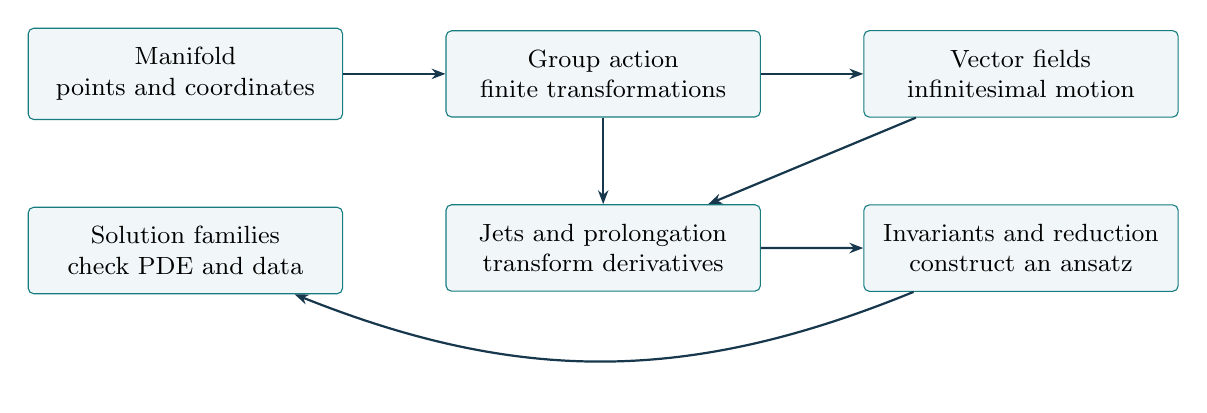
\begin{tikzpicture}[node distance=11mm and 13mm]
\node[main,text width=35mm] (geo) {Manifold\\points and coordinates};
\node[main,text width=35mm,right=of geo] (act) {Group action\\finite transformations};
\node[main,text width=35mm,right=of act] (vf) {Vector fields\\infinitesimal motion};
\node[main,text width=35mm,below=of act] (jet) {Jets and prolongation\\transform derivatives};
\node[main,text width=35mm,below=of geo] (sol) {Solution families\\check PDE and data};
\node[main,text width=35mm,below=of vf] (red) {Invariants and reduction\\construct an ansatz};
\draw[arr] (geo)--(act);\draw[arr] (act)--(vf);
\draw[arr] (vf)--(jet);\draw[arr] (jet)--(red);\draw[arr] (red) to[bend left=22] (sol);
\draw[arr] (act)--(jet);
\end{tikzpicture}
\caption{The learning route. Finite transformations also create new solutions directly, without a reduction.}
\end{figure}

\section{Manifolds: local coordinates with reliable overlap}\label{sec:manifolds}
\source{Section 2.1, printed pp.~4--5}

\subsection{Open sets, charts, and smooth changes of coordinates}
A topology specifies which subsets are open: the empty set and the whole space are open, arbitrary unions of open sets are open, and finite intersections of open sets are open. In $\R^n$, an open set contains a small Euclidean ball around each of its points. A map is continuous when inverse images of open sets are open. A homeomorphism is a bijection that is continuous in both directions. It is an exact topological identification; the phrase ``deformation without tearing'' is only a visual guide.

A chart on an $m$-dimensional manifold is a homeomorphism
\[
\chi:U\longrightarrow V,\qquad U\subset M\text{ open},\quad V\subset\R^m\text{ open}.
\]
The point $p\in U$ and its coordinate tuple $\chi(p)$ represent the same location in different spaces. An atlas is a collection of charts covering $M$. On an overlap, a point with coordinates $a=\chi_\alpha(p)$ has coordinates
\[
b=\chi_\beta(p)=\chi_\beta\circ\chi_\alpha^{-1}(a).
\]
This transition map, and its reverse, must be smooth. The transition is defined only on $\chi_\alpha(U_\alpha\cap U_\beta)$, not on the whole chart image unless the domains agree.

\begin{definition}[Smooth manifold]
A smooth manifold is a Hausdorff, second-countable topological space that is locally homeomorphic to open subsets of a fixed $\R^m$, equipped with a smooth atlas. Second-countable means that a countable family of open sets generates all open sets by unions. An atlas determines a maximal compatible smooth atlas; it is the smooth structure, not a particular choice of coordinates, that matters.
\end{definition}
A map $F:M\to N$ between smooth manifolds is smooth if every applicable coordinate expression $\psi\circ F\circ\chi^{-1}$ is smooth. A diffeomorphism is a smooth bijection with a smooth inverse. This is stronger than a homeomorphism: $s\mapsto s^3$ is a smooth homeomorphism of $\R$, but its cube-root inverse is not differentiable at zero.

Connectedness is optional. A manifold need not be globally a deformation of $\R^m$. The circle is compact and $\R$ is not. Also, a hypersurface means codimension one in an ambient space, not simply a manifold of dimension at least three.

\subsection{The third condition: Hausdorff separation}\label{sec:hausdorff}
The report's third property says the following. For distinct points $p\in U_\alpha$ and $q\in U_\beta$, find coordinate-open neighbourhoods
\[
\chi_\alpha(p)\in W\subset V_\alpha,
\qquad \chi_\beta(q)\in\widehat W\subset V_\beta
\]
such that their inverse images do not meet:
\begin{equation}\label{eq:hausdorff}
\chi_\alpha^{-1}(W)\cap\chi_\beta^{-1}(\widehat W)=\varnothing.
\end{equation}
Here $\chi^{-1}(W)$ means all points whose coordinates lie in $W$. The sets to separate are on $M$. Two numerical coordinate patches can overlap in $\R^m$ even when they represent disjoint parts of $M$.

\begin{example}[An explicit choice on the line]
Take $M=\R$, $p=0$, $q=3$, with the identity chart. Choose $W=(-1,1)$ and $\widehat W=(2,4)$. Their inverse images are the same disjoint intervals. More generally, for $p\ne q$ in $\R^n$, balls of radius $\|p-q\|/3$ around them are disjoint. Every subspace of Euclidean space inherits the Hausdorff property.
\end{example}

\begin{figure}[htbp]\centering
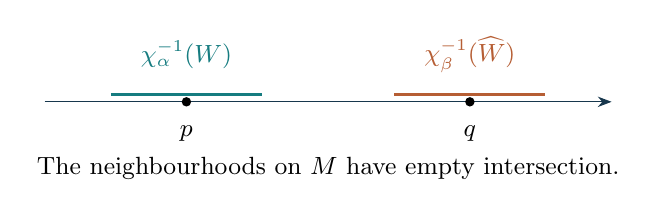
\begin{tikzpicture}[x=1.2cm,y=1cm]
\draw[->,ink] (-1.5,0)--(4.5,0);
\draw[accent,very thick] (-.8,.09)--(.8,.09);
\draw[warm,very thick] (2.2,.09)--(3.8,.09);
\fill (0,0) circle (1.7pt) node[below=5pt]{$p$};
\fill (3,0) circle (1.7pt) node[below=5pt]{$q$};
\node[accent] at (0,.6){$\chi_\alpha^{-1}(W)$};
\node[warm] at (3,.6){$\chi_\beta^{-1}(\widehat W)$};
\node at (1.5,-.85){The neighbourhoods on $M$ have empty intersection.};
\end{tikzpicture}
\caption{Hausdorff separation is a condition on distinct points and their neighbourhoods. It is not a differentiability condition.}
\end{figure}

\begin{example}[Why local coordinates alone do not suffice]
Take two copies of $\R$ and identify their points with the same nonzero coordinate, but keep two distinct origins $0_a,0_b$. Each origin has a neighbourhood looking like an interval, so the resulting ``line with two origins'' is locally Euclidean. Nevertheless, every neighbourhood of $0_a$ meets every neighbourhood of $0_b$ at shared nonzero points. The sequence $1/n$ converges to both origins. The space fails~\eqref{eq:hausdorff} and is excluded from our manifolds.
\end{example}
The Hausdorff property gives uniqueness of limits: if a sequence converged to distinct $p$ and $q$, it would eventually lie in two disjoint neighbourhoods at once. It also ensures compact subsets are closed. These are basic tools for doing geometry consistently.

\subsection{A complete two-chart calculation on the circle}
Let $S^1=\{(x,y):x^2+y^2=1\}$. Delete the north pole for $U_N$ and the south pole for $U_S$, and define
\[
\chi_N(x,y)=\frac{x}{1-y},\qquad \chi_S(x,y)=\frac{x}{1+y}.
\]
To invert the second chart, set $s=x/(1+y)$, so $x=s(1+y)$. Substitute into $x^2+y^2=1$ and factor:
\[
s^2(1+y)^2+y^2-1=(1+y)\bigl(s^2(1+y)+y-1\bigr)=0.
\]
The deleted south pole would have $1+y=0$. On the chart, solve the other factor:
\[
y=\frac{1-s^2}{1+s^2},\qquad x=\frac{2s}{1+s^2}.
\]
Thus
\[
\chi_S^{-1}(s)=\left(\frac{2s}{1+s^2},\frac{1-s^2}{1+s^2}\right),\quad
\chi_N\circ\chi_S^{-1}(s)=\frac1s\quad(s\ne0).
\]
The overlap excludes both poles, which explains $s\ne0$. All derivatives of $1/s$ exist there. The two chart domains cover the circle, and its Hausdorff property follows from $S^1\subset\R^2$.

\begin{figure}[htbp]\centering
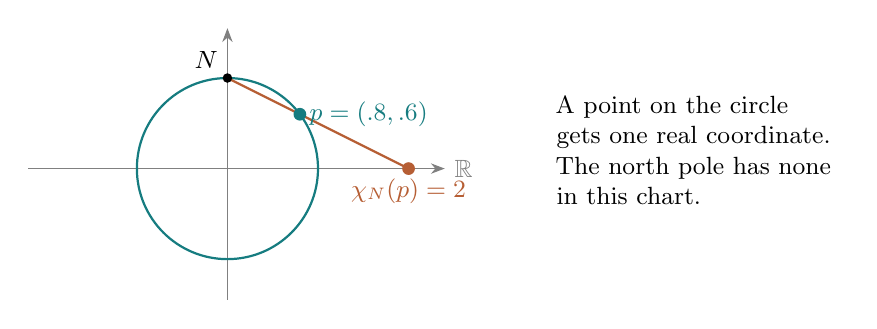
\begin{tikzpicture}[scale=1.15]
\draw[->,gray] (-2.2,0)--(2.4,0) node[right]{$\R$};
\draw[->,gray] (0,-1.45)--(0,1.55);
\draw[accent,thick] (0,0) circle (1);
\coordinate (N) at (0,1);\coordinate (P) at (.8,.6);\coordinate (S) at (2,0);
\draw[warm,thick] (N)--(S);
\fill (N) circle (1.5pt) node[above left]{$N$};
\fill[accent] (P) circle (2pt) node[right]{$p=(.8,.6)$};
\fill[warm] (S) circle (2pt) node[below]{$\chi_N(p)=2$};
\node[align=left,text width=3.6cm] at (5.2,.2){A point on the circle\\gets one real coordinate.\\The north pole has none\\in this chart.};
\end{tikzpicture}
\caption{Stereographic coordinates. The line from $(0,1)$ through $(x,y)$ meets the horizontal axis at $x/(1-y)$.}
\end{figure}

\subsection{Products of manifolds}\label{sec:products}
The Cartesian product is the set of ordered pairs:
\[
M\times N=\{(p,q):p\in M,\ q\in N\}.
\]
It does not multiply the points numerically. If $\chi:U\to\R^m$ and $\psi:V\to\R^n$ are charts, a product chart is
\[
\chi\times\psi:U\times V\longrightarrow\R^{m+n},\qquad
(p,q)\longmapsto(\chi(p),\psi(q)).
\]
Its transition map applies the two transition maps separately, so it is smooth. Hausdorff separation follows by separating a coordinate in which two pairs differ; products of countable bases are countable. Hence
\[
\boxed{\dim(M\times N)=\dim M+\dim N.}
\]
For example, $\R\times\R=\R^2$, and $(x,t,u)$ is a point of $\R^2_{x,t}\times\R_u$. The torus $S^1\times S^1$ has two independent angles. Its natural pair-of-circles representation lies in $\R^4$; the familiar doughnut in $\R^3$ is a different embedding of the same abstract manifold:
\[
(\theta,\phi)\longmapsto
\bigl((R+r\cos\phi)\cos\theta,(R+r\cos\phi)\sin\theta,r\sin\phi\bigr),
\quad R>r>0.
\]
Angles are taken modulo $2\pi$; use open angle intervals for local charts.

\begin{figure}[htbp]\centering
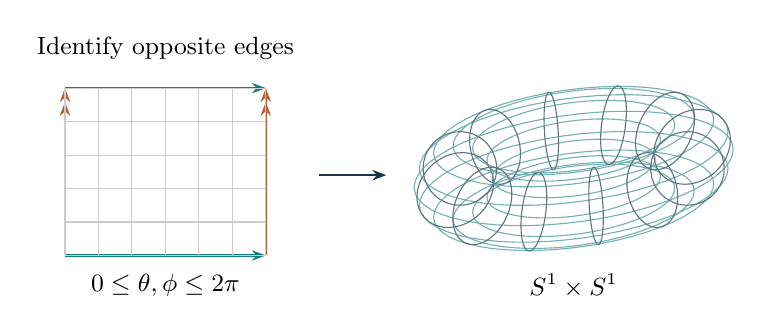
\begin{tikzpicture}[scale=.85]
\begin{scope}
\draw[accent,thick,->] (0,0)--(3,0);\draw[accent,thick,->] (0,2.5)--(3,2.5);
\draw[warm,thick,->>] (0,0)--(0,2.5);\draw[warm,thick,->>] (3,0)--(3,2.5);
\draw[gray!40,step=.5] (0,0) grid (3,2.5);
\node at (1.5,-.45){$0\le\theta,\phi\le2\pi$};
\node at (1.5,3.1){Identify opposite edges};
\end{scope}
\draw[arr] (3.8,1.2)--(4.8,1.2);
\begin{scope}[shift={(7.6,1.3)},x={(1cm,0cm)},y={(.35cm,.38cm)},z={(0cm,1cm)}]
\foreach \v in {0,30,...,330}{
\draw[accent!60,thin,samples=55,domain=0:360,variable=\s] plot ({(1.7+.55*cos(\v))*cos(\s)},{(1.7+.55*cos(\v))*sin(\s)},{.55*sin(\v)});}
\foreach \v in {0,30,...,330}{
\draw[ink!70,thin,samples=40,domain=0:360,variable=\s] plot ({(1.7+.55*cos(\s))*cos(\v)},{(1.7+.55*cos(\s))*sin(\v)},{.55*sin(\s)});}
\end{scope}
\node at (7.6,-.45){$S^1\times S^1$};
\end{tikzpicture}
\caption{Two periodic coordinates produce a torus. The rectangle is a gluing picture, not one global chart. A product is a new manifold, not a group operation.}
\end{figure}
If $G$ is a Lie group, $G\times G$ is merely the \emph{domain} of its multiplication map $\mu$. If $G,H$ are both groups, one may additionally define the product-group law $(g,h)(g',h')=(gg',hh')$. These are two uses of the same product set with different maps on it.

\section{Derivatives, rank, and parametrized submanifolds}\label{sec:maps}
\source{Definitions 2.4--2.5 and 2.22}
\subsection{The derivative and what rank counts}\label{sec:rank}
For $F:M^m\to N^n$, the derivative at $p$ is a linear map
\[
dF_p:T_pM\longrightarrow T_{F(p)}N.
\]
In coordinates it is represented by the $n\times m$ Jacobian
\[
J_F(p)=\left(\frac{\partial F^i}{\partial x^j}(p)\right),\qquad
F(p+h)=F(p)+J_F(p)h+o(\|h\|).
\]
The rank is the dimension of the image of this linear map: the number of independent output directions visible to first order. It can be found by row reduction, independent columns, or the largest nonzero minor. It is an integer between $0$ and $\min(m,n)$.

\begin{example}[Constant rank, nonconstant Jacobian]
Let $F(s,t)=(s^2+t,2s^2+2t)$. Then
\[
J_F(s,t)=\begin{pmatrix}2s&1\\4s&2\end{pmatrix}.
\]
The second row is twice the first, so the rank is at most one. The second column is $(1,2)^T\ne0$, so the rank is at least one. Therefore the rank is exactly one everywhere, although the entries depend on $s$. The image lies on the line $y=2x$.
\end{example}

\begin{example}[A rank change]
For $F(x,y)=(x,y^2)$,
\[
J_F=\begin{pmatrix}1&0\\0&2y\end{pmatrix},\qquad
\rank J_F=\begin{cases}2,&y\ne0,\\1,&y=0.\end{cases}
\]
The derivative loses the vertical direction on $y=0$. The map is smooth everywhere but is not a constant-rank map on the whole plane. It is a local diffeomorphism on either half-plane $y>0$ or $y<0$.
\end{example}

\begin{figure}[htbp]\centering
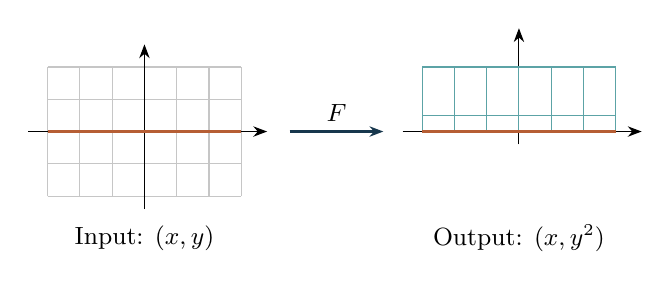
\begin{tikzpicture}[scale=.82]
\draw[gray!45,step=.5] (-1.5,-1) grid (1.5,1);
\draw[->] (-1.8,0)--(1.9,0);\draw[->] (0,-1.2)--(0,1.35);
\draw[warm,very thick] (-1.5,0)--(1.5,0);
\node at (0,-1.65){Input: $(x,y)$};
\draw[arr] (2.25,0)--node[above]{$F$}(3.7,0);
\begin{scope}[shift={(5.8,0)}]
\draw[->] (-1.8,0)--(1.9,0);\draw[->] (0,-.2)--(0,1.6);
\foreach \x in {-1.5,-1,-.5,0,.5,1,1.5}{\draw[accent!70] (\x,0)--(\x,1);}
\foreach \y in {0,.25,1}{\draw[accent!70] (-1.5,\y)--(1.5,\y);}
\draw[warm,very thick] (-1.5,0)--(1.5,0);
\node at (0,-1.65){Output: $(x,y^2)$};
\end{scope}
\end{tikzpicture}
\caption{The upper and lower halves fold onto the same half-plane. At the highlighted line, the first-order vertical motion vanishes. Constant rank excludes this change of local behaviour.}
\end{figure}

A change of charts replaces $J_F$ by $A J_F B$, where $A$ and $B$ are invertible Jacobians of coordinate changes. Multiplication by invertible matrices does not change rank. Thus rank is a property of $F$, not of the coordinates used to compute it.

\begin{proposition}[Constant-rank theorem, usable form]
If $\rank dF=r$ throughout a neighbourhood of $p$, suitable smooth coordinates in the domain and codomain put the map into the form
\[
(s^1,\ldots,s^m)\longmapsto(s^1,\ldots,s^r,0,\ldots,0).
\]
The zero entries may require translating the output coordinates.
\end{proposition}
This explains the purpose of the hypothesis. Locally the map transmits $r$ coordinates and ignores $m-r$ of them. Its nonempty local fibres have dimension $m-r$. For PDE symmetry, such coordinates let us distinguish motion along orbits from independent invariants. We do \emph{not} impose constant rank on every smooth function in the problem; we check it on the relevant map and region.

\subsection{Regular values and constraint surfaces}\label{sec:levelsets}
For $F:M^m\to\R^k$, a value $c$ is regular if $dF_p$ is surjective (rank $k$) at every $p\in F^{-1}(c)$. Then the regular-level-set theorem gives
\[
F^{-1}(c)\text{ an embedded submanifold of dimension }m-k,
\qquad T_pF^{-1}(c)=\ker dF_p.
\]
For $F(x,y)=x^2+y^2$, $dF=(2x,2y)$. On $F^{-1}(1)$ it has rank one, so the unit circle is one-dimensional. The value zero is critical: its level set is a single point, and the dimension formula $2-1$ does not apply. A defining function can also be unnecessarily singular: $(x^2+y^2-1)^2=0$ describes the same smooth circle but its derivative vanishes on that circle. Replace it by $x^2+y^2-1=0$ before applying a rank-based tangency test.

\subsection{Immersion, embedding, and parameter space}\label{sec:immersion}
A parameter space $P$ is itself a manifold. Its points label locations on an image in another manifold:
\[
F:P^n\longrightarrow M^m,\qquad a\longmapsto F(a),\qquad n\le m.
\]
A local parameter space usually looks like an open interval, disk or box in $\R^n$. Globally it can be a circle or torus. It is not automatically a tangent space and is not necessarily a Lie group.

\begin{definition}[Immersion and embedding]
$F:P\to M$ is an immersion if $dF_a$ is injective for every $a$, equivalently $\rank dF_a=n=\dim P$. It is an embedding if it is also a homeomorphism onto its image equipped with the subspace topology of $M$. In particular an embedding is injective. An immersed submanifold can be described as a manifold $N$ whose inclusion into $M$ is an injective immersion; its topology can be finer than the subspace topology.
\end{definition}
The report's Definition 2.5 uses a one-to-one immersion to give its image a manifold structure transported from the parameter space. This is a convention for \emph{immersed submanifolds}; it is not a definition of every immersion. Immersions as maps need not be one-to-one.

\begin{example}[A parabola from an interval]
Take $P=\R$, $F(s)=(s,s^2)$. Its Jacobian is the column $(1,2s)^T$, of rank one for all $s$. The map is injective, and the inverse on its image is the continuous projection $(x,y)\mapsto x$. It is an embedding. Near any point, one number $s$ locates a point on this curve in a two-dimensional ambient space.
\end{example}

\begin{example}[Self-intersection does not invalidate an immersion]
Take $P=S^1$, using angle $\theta$ modulo $2\pi$, and set
\[
F(\theta)=(\sin\theta,\sin2\theta),\qquad F'(\theta)=(\cos\theta,2\cos2\theta).
\]
The two derivative components never vanish together, so this is an immersion. However $F(0)=F(\pi)=(0,0)$. Its image is a figure-eight; with its subspace topology, the crossing is not locally an interval. The smooth domain is still a circle. For comparison, $C(s)=(s^2,s^3)$ is injective but $C'(0)=0$: it fails to be an immersion at its cusp.
\end{example}

\begin{figure}[htbp]\centering
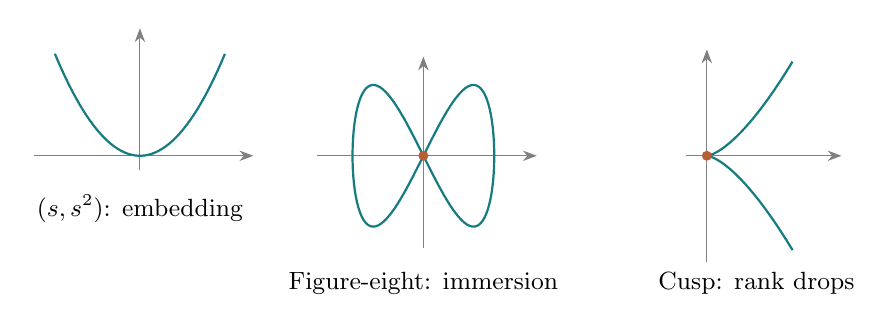
\begin{tikzpicture}[scale=.9]
\begin{scope}[shift={(-4,0)}]
\draw[->,gray] (-1.5,0)--(1.6,0);\draw[->,gray] (0,-.2)--(0,1.8);
\draw[accent,thick,domain=-1.2:1.2,samples=50] plot (\x,{\x*\x});
\node at (0,-.75){$(s,s^2)$: embedding};
\end{scope}
\begin{scope}
\draw[->,gray] (-1.5,0)--(1.6,0);\draw[->,gray] (0,-1.3)--(0,1.4);
\draw[accent,thick,domain=0:360,samples=120,variable=\s] plot ({sin(\s)},{sin(2*\s)});
\fill[warm] (0,0) circle (2pt);
\node at (0,-1.8){Figure-eight: immersion};
\end{scope}
\begin{scope}[shift={(4,0)}]
\draw[->,gray] (-.3,0)--(1.9,0);\draw[->,gray] (0,-1.5)--(0,1.5);
\draw[accent,thick,domain=-1.1:1.1,samples=60,variable=\s] plot ({\s*\s},{\s*\s*\s});
\fill[warm] (0,0) circle (2pt);
\node[align=center] at (.7,-1.8){Cusp: rank drops};
\end{scope}
\end{tikzpicture}
\caption{A parameterized image, its derivative, and its topology are different pieces of information. Full derivative rank prevents a cusp, but alone does not prevent a self-intersection.}
\end{figure}
An injective immersion need not be an embedding: for irrational $a$, the map $s\mapsto(e^{is},e^{ias})$ injects $\R$ densely into $S^1\times S^1$. Its derivative has rank one, but its inverse is not continuous for the image's subspace topology. A proper injective immersion, or an injective immersion from a compact manifold into a Hausdorff manifold, is an embedding.

\section{Lie groups and their actions}\label{sec:groups}
\source{Section 2.2}
\subsection{The axioms, with the compatibility made explicit}
A group is a set $G$ with a multiplication $\mu:G\times G\to G$ satisfying associativity, an identity $e$, and inverses. Closure is already encoded by the codomain $G$. In symbols, for all $g,h,k\in G$,
\[
(gh)k=g(hk),\qquad eg=ge=g,\qquad gg^{-1}=g^{-1}g=e.
\]
 A Lie group is additionally a smooth manifold, with smooth multiplication and inversion $g\mapsto g^{-1}$. Counting ``four plus four'' conditions can help a checklist, but misses the essential compatibility: the group operations must be smooth in the chosen manifold structure.

\begin{tabularx}{\linewidth}{@{}p{.27\linewidth}Y@{}}
\toprule Object & Meaning \\
\midrule $G$ & A manifold with a group law; it is not a map.\\
$\mu:G\times G\to G$ & A smooth map combining two group elements into one.\\
$\Phi:G\times M\to M$ & An action: a group element moves a point of another manifold.\\
$\Phi_g:M\to M$ & The transformation obtained by fixing $g$.\\
$f:G\to H$ & A Lie group homomorphism if it is smooth and $f(gh)=f(g)f(h)$.\\
\bottomrule
\end{tabularx}
For $(\R,+)$, $\mu(a,b)=a+b$ and inversion is $a\mapsto-a$. For $\R_{>0}$ under multiplication, $\mu(a,b)=ab$ and inversion is $1/a$. The map $a\mapsto e^a$ is a Lie group isomorphism between these examples because $e^{a+b}=e^ae^b$, and its smooth inverse is $\log$.

\subsection{What is actually isomorphic to \texorpdfstring{$\R^{n^2}$}{R to the n squared}?}\label{sec:gl}
Let $M_n(\R)$ denote \emph{all} real $n\times n$ matrices. Listing their entries defines a linear isomorphism
\[
\operatorname{vec}:M_n(\R)\longrightarrow\R^{n^2}.
\]
For $n=2$,
\[
\begin{pmatrix}a&b\\c&d\end{pmatrix}\longleftrightarrow(a,b,c,d).
\]
It preserves matrix addition and scalar multiplication, and is also a diffeomorphism of the underlying manifolds. But the invertible matrices correspond only to an open subset:
\[
\GL(2,\R)\longleftrightarrow
\{(a,b,c,d)\in\R^4:ad-bc\ne0\}.
\]
For general $n$, the determinant is a continuous polynomial, and $\R\setminus\{0\}$ is open. Therefore
\[
\GL(n,\R)=\det^{-1}(\R\setminus\{0\})
\]
is open in $M_n(\R)$ and is an $n^2$-dimensional manifold. A single global chart maps it to that open subset of $\R^{n^2}$.

\begin{correction}{The distinction in Example 2.10}
$M_n(\R)\cong\R^{n^2}$ as vector spaces. $\GL(n,\R)$ is identified with an \emph{open subset} of $\R^{n^2}$ as a manifold. There is no asserted group isomorphism from matrix multiplication to ordinary addition on $\R^{n^2}$. Indeed $\GL(n,\R)$ has positive- and negative-determinant components, whereas $\R^{n^2}$ is connected.
\end{correction}
For example, $\operatorname{vec}(2I\cdot3I)=\operatorname{vec}(6I)$ while $\operatorname{vec}(2I)+\operatorname{vec}(3I)=\operatorname{vec}(5I)$. For $n\ge2$ there is also noncommutativity, unlike addition.

To check the Lie group structure, compute
\[
\begin{pmatrix}a&b\\c&d\end{pmatrix}
\begin{pmatrix}e&f\\g&h\end{pmatrix}
=\begin{pmatrix}ae+bg&af+bh\\ce+dg&cf+dh\end{pmatrix},
\]
a polynomial in eight entries. Inversion is
\[
\begin{pmatrix}a&b\\c&d\end{pmatrix}^{-1}
=\frac1{ad-bc}\begin{pmatrix}d&-b\\-c&a\end{pmatrix}.
\]
It is smooth where $ad-bc\ne0$. In general use $A^{-1}=\operatorname{adj}(A)/\det A$. Nonzero determinant is not itself a proof of smoothness; this formula supplies the proof.

\subsection{Global actions and the space being acted on}
An action is a smooth map $\Phi:G\times M\to M$, written $g\cdot p$, such that
\[
e\cdot p=p,\qquad g\cdot(h\cdot p)=(gh)\cdot p.
\]
Each $\Phi_g$ is a diffeomorphism with inverse $\Phi_{g^{-1}}$. The dimension of $G$ counts group parameters; the dimension of $M$ counts coordinates of the points moved. They need not agree.
For example, $\SO(2)$ is a one-dimensional group acting on the two-dimensional plane by
\[
R_\theta\binom{x}{y}=
\begin{pmatrix}\cos\theta&-\sin\theta\\\sin\theta&\cos\theta\end{pmatrix}\binom{x}{y}.
\]
$\SO(2)$ is isomorphic to the unit complex numbers under multiplication. The circle of group elements and a circular orbit in the plane play different roles, even though both are circles.

\subsection{Local actions and their domains}\label{sec:local}
Some transformations can be followed only for a limited parameter interval. A local action is a smooth map
\begin{equation}\label{eq:local-action}
\Phi:\mathcal U\longrightarrow M,\qquad
\{e\}\times M\subset\mathcal U\subset G\times M,
\end{equation}
with $\mathcal U$ open and the identity, inverse and composition laws valid wherever the relevant pairs and products are defined. We use the usual local-flow convention: for each point the admissible parameter interval contains zero. The report uses $U$ for $\mathcal U$; here $\mathcal U$ avoids confusion with the dependent-variable range.

The phrase \emph{domain of definition of the group action} means the set of \emph{admissible pairs} $(g,p)$. It is not just a subset of $M$. Fixing $p$ leaves the permissible group elements; fixing $g$ leaves the permissible starting points.

\begin{example}[A local action calculated from an ODE]
On $M=\R$ solve $\dot q=q^2$, $q(0)=q_0$. For $q_0\ne0$, integration gives $-1/q=\varepsilon-1/q_0$, so
\[
\Phi_\varepsilon(q)=\frac{q}{1-\varepsilon q},\qquad
\mathcal U=\{(\varepsilon,q)\in\R^2:1-\varepsilon q>0\}.
\]
The same formula fixes $q=0$. The strict inequality selects the maximal interval connected to zero; it does not jump through a pole. For $q=2$, admissible parameters satisfy $\varepsilon<1/2$. For $\varepsilon=1$, admissible starting points satisfy $q<1$.
\[
\Phi_\varepsilon(\Phi_\delta(q))
=\frac{q/(1-\delta q)}{1-\varepsilon q/(1-\delta q)}
=\frac{q}{1-(\varepsilon+\delta)q}
=\Phi_{\varepsilon+\delta}(q)
\]
whenever the sequential actions are defined. The inverse is $\Phi_{-\varepsilon}$ on the image. At $q=2,\varepsilon=1/2$ the solution blows up, so the action cannot be global.
\end{example}

\begin{figure}[htbp]\centering
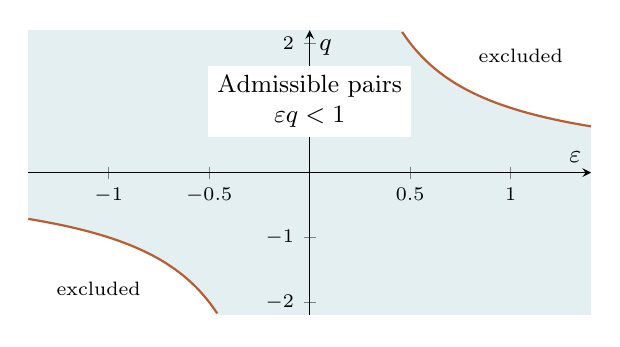
\begin{tikzpicture}
\begin{axis}[width=.72\linewidth,height=5.2cm,xmin=-1.4,xmax=1.4,ymin=-2.2,ymax=2.2,axis lines=middle,axis background/.style={fill=accent!12},xlabel={$\varepsilon$},ylabel={$q$},samples=90,tick label style={font=\scriptsize}]
\addplot[draw=none,fill=white,domain=.454545:1.4] {1/x} -- (axis cs:1.4,2.2) -- cycle;
\addplot[draw=none,fill=white,domain=-1.4:-.454545] {1/x} -- (axis cs:-1.4,-2.2) -- cycle;
\addplot[warm,thick,domain=.46:1.4]{1/x};
\addplot[warm,thick,domain=-1.4:-.46]{1/x};
\node[fill=white,align=center,font=\small] at (axis cs:0,1.1){Admissible pairs\\$\varepsilon q<1$};
\node[font=\scriptsize] at (axis cs:1.05,1.8){excluded};
\node[font=\scriptsize] at (axis cs:-1.05,-1.8){excluded};
\end{axis}
\end{tikzpicture}
\caption{The action domain is the open region $\varepsilon q<1$, including both axes. The hyperbola is excluded. The shaded region consists of admissible pairs; the two white corner regions are excluded.}
\end{figure}

\subsection{Orbits, stabilizers, and regular actions}\label{sec:regular-actions}
The orbit of $p$ consists of points reachable by the action (or admissible successive local transformations). For a global action,
\[
G\cdot p=\{g\cdot p:g\in G\},\qquad G_p=\{g:g\cdot p=p\}.
\]
$G_p$ is the stabilizer. For a smooth global action its orbits are immersed submanifolds, modeled on $G/G_p$, and
\[
\dim(G\cdot p)=\dim G-\dim G_p.
\]
They need not be embedded. Under plane rotations, the origin is a zero-dimensional orbit, and every other orbit is a circle $x^2+y^2=r^2$. If $r$ is a distance, write $r^2$ on the right, not $r$.

The word \emph{regular} for actions needs a definition. In Olver's convention~\cite{olvernotes}, an action is \emph{semi-regular} if all orbits have the same dimension. It is \emph{regular} if, additionally, every point has arbitrarily small neighbourhoods whose intersection with each orbit is connected. Local orbit pieces then have coordinates
\[
(s^1,\ldots,s^r,z^1,\ldots,z^{m-r}),
\]
where $s$ describes motion along an orbit and $z$ labels orbit slices. A constant orbit dimension already gives local foliation charts; the stronger condition prevents an orbit repeatedly returning in disconnected slices of the same small chart.

For rotations, the action is regular on $\R^2\setminus\{0\}$, with a local angle as orbit coordinate and radius as invariant. On all of $\R^2$ the orbit dimension changes at zero. The irrational torus flow $(\theta,\phi)\mapsto(\theta+\varepsilon,\phi+a\varepsilon)$ has one-dimensional dense orbits; it is semi-regular but not regular in this convention. Its local invariant $\phi-a\theta$ is not a globally single-valued function on the torus. A global quotient manifold needs further hypotheses; a free proper action is a standard sufficient condition.

\begin{idea}{Do not test regularity of an action using the wrong map}
The full action map $\Phi:G\times M\to M$ is a submersion: varying $p$ at fixed $g$ already gives the derivative of a diffeomorphism. Its rank is always $\dim M$, even for rotation at the origin. Orbit dimension is instead the rank of the orbit map $g\mapsto g\cdot p$, or the span of infinitesimal generators at $p$.
\end{idea}

\subsection{A dictionary for the word ``regular''}\label{sec:regular-dictionary}
\begin{longtable}{@{}>{\raggedright\arraybackslash}p{.27\linewidth}>{\raggedright\arraybackslash}p{.67\linewidth}@{}}
\toprule Phrase & Meaning in context \\
\midrule\endhead
Regular map in the report, Definition 2.4 & Its derivative has constant rank on the stated domain. This is stronger than smoothness, but need not mean maximal rank.\\
Immersion of an $n$-manifold & Rank $n$ at every point: full column rank. A parametrization loses no tangent direction.\\
Submersion to an $n$-manifold & Rank $n$ at every point: full row rank. Every target tangent direction can be reached.\\
Regular value of $F:M\to\R^k$ & $\rank dF=k$ at every point of the corresponding level set. The map may have critical points on other levels.\\
Regular equation $F=0$ & The defining functions have independent differentials on the zero set. For one scalar equation, $dF\ne0$ there.\\
Semi-regular / regular action & Constant orbit dimension / the additional no-return condition described above. Smoothness of the action alone is insufficient.\\
Regular submanifold & In some transformation-group texts, an embedded submanifold with the subspace topology. State the convention; it is not a new kind of Jacobian.\\
Fully regular PDE system & Regular defining equations plus local solvability: permitted equation jets can be realized by local solutions. This matters in the necessity direction of the symmetry criterion.\\
Regular function or map in Etingof's notes & A function or map of the chosen differentiability class, such as smooth or analytic. This is \emph{not} the report's constant-rank definition.\\
Regularity of a PDE solution & How many derivatives, or which function-space properties, a solution has. It is unrelated to constant Jacobian rank.\\
Regular holonomic $\mathcal D$-module & A technical condition on singularities in a different theory; no constant-rank interpretation is intended. See Section~\ref{sec:advanced}.\\
\bottomrule
\end{longtable}
The blanket convention in the report's Remark 2.6 should not be read as a theorem that all smooth maps are regular or all manifolds connected. We state the needed rank, domain and connectedness hypotheses at the point of use.

\section{Vectors, tangent spaces, vector fields, and flows}\label{sec:vectors}
\source{Section 2.3, printed pp.~8--11}
\subsection{Which object contains which?}
A real vector space is a set whose elements can be added and multiplied by real scalars, satisfying the usual linear-algebra axioms. A vector is one element of such a space. On a curved manifold, velocities based at a \emph{fixed point} form a vector space, the tangent space $T_pM$. It has dimension $\dim M$. There is generally no intrinsic addition of a point $p$ to a point $q$, or of a tangent vector at $p$ to one at $q$.

\begin{tabularx}{\linewidth}{@{}p{.25\linewidth}p{.26\linewidth}Y@{}}
\toprule Object & What one element is & Example \\
\midrule $M$ & A point $p$ & A point on a circle.\\
$T_pM$ & A velocity based at $p$ & A tangent arrow at that point.\\
$TM=\bigsqcup_{p\in M}T_pM$ & A pair $(p,v)$ & A point and an arrow based there.\\
$X\in\mathfrak X(M)$ & A smooth choice $p\mapsto X_p$ & One tangent arrow at every point.\\
$\mathfrak X(M)$ & A vector field & An infinite-dimensional real vector space in positive dimension.\\
$\g=T_eG$ & An infinitesimal group element & A finite-dimensional space for a finite-dimensional Lie group.\\
\bottomrule
\end{tabularx}
The tangent bundle $TM$ is a manifold of dimension $2\dim M$ and a vector bundle over $M$. Its projection is $\pi(p,v)=p$. A vector field is a smooth section $X:M\to TM$ with $\pi\circ X=\id_M$. The fibres are vector spaces; the entire tangent bundle is not generally one vector space.

\subsection{A tangent vector as velocity and as a derivative}
Let $\gamma:(-a,a)\to M$ be a smooth curve with $\gamma(0)=p$. In a chart $x^1,\ldots,x^m$, its velocity is
\[
v=\dot\gamma(0)=\sum_i\left.\frac{d(x^i\circ\gamma)}{ds}\right|_{s=0}\partial_{x^i}\big|_p.
\]
For a smooth function $f$, the chain rule says
\[
v(f)=\left.\frac{d}{ds}f(\gamma(s))\right|_{s=0}
=\sum_i v^i\partial_{x^i}f(p).
\]
Thus $\partial_{x^i}|_p$ is both a coordinate basis vector and the operation of taking the corresponding partial derivative at $p$. This is why differential-operator notation represents arrows correctly.

For the unit circle, $\gamma(\theta)=(\cos\theta,\sin\theta)$ gives the field
\[
X=-y\partial_x+x\partial_y.
\]
At $p=(1,0)$, $X_p=(0,1)$; at $q=(0,1)$, $X_q=(-1,0)$. The tangent space at $(x,y)\in S^1$ is
\[
T_{(x,y)}S^1=\{(a,b):xa+yb=0\},
\]
a one-dimensional line of allowable velocities, not the circle itself.

\begin{figure}[htbp]\centering
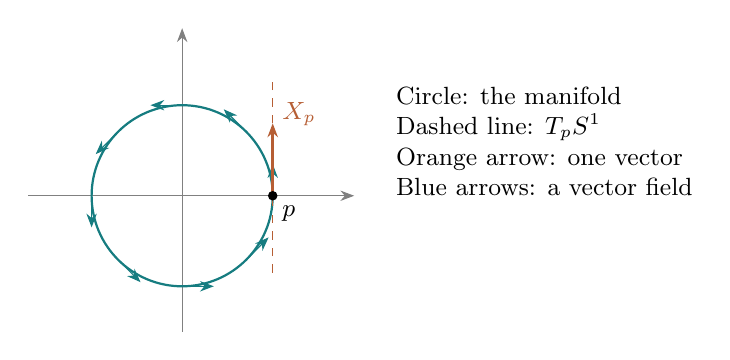
\begin{tikzpicture}[scale=1.15]
\draw[gray,->] (-1.7,0)--(1.9,0);\draw[gray,->] (0,-1.5)--(0,1.85);
\draw[accent,thick] (0,0) circle (1);
\foreach \a in {0,45,...,315}{\draw[accent,->] ({cos(\a)},{sin(\a)})--({cos(\a)-.35*sin(\a)},{sin(\a)+.35*cos(\a)});}
\draw[warm,dashed] (1,-.85)--(1,1.3);
\draw[warm,very thick,->] (1,0)--(1,.8);
\fill (1,0) circle (1.5pt) node[below right]{$p$};
\node[warm,right] at (1,.9){$X_p$};
\node[align=left] at (4.0,.6){Circle: the manifold\\Dashed line: $T_pS^1$\\Orange arrow: one vector\\Blue arrows: a vector field};
\end{tikzpicture}
\caption{A tangent space contains every multiple of its basis vector at one point. A vector field selects one vector in each tangent space. The affine tangent line is drawn through $p$ to visualize the abstract space.}
\end{figure}

\subsection{Why vector fields form a vector space}
For constants $a,b\in\R$, define $(aX+bY)_p=aX_p+bY_p$. Both arrows on the right live in $T_pM$, so the operation is meaningful. One may also multiply by a smooth function: $(fX)_p=f(p)X_p$. This makes $\mathfrak X(M)$ a module over $C^\infty(M)$ as well as a vector space over $\R$.

On a coordinate region in $\R^3$, every field is $a\partial_x+b\partial_t+c\partial_u$ with smooth coefficient functions. This is a basis of three fields over \emph{functions}. Over \emph{constant scalars}, the fields $\partial_x,x\partial_x,x^2\partial_x,\ldots$ are linearly independent, so the space is infinite-dimensional. The six heat generators can therefore be independent vector fields even though each tangent space has only dimension three.

Every vector field is a derivation:
\[
X(fg)=X(f)g+fX(g).
\]
A derivation of the full algebra of smooth functions corresponds to a smooth vector field. A derivation becomes a \emph{symmetry generator of a particular equation} only after passing that equation's invariance test. For example, $\partial_x$ is a vector field everywhere but is not a symmetry of $u_t=xu$ under plain $x$-translation.

\subsection{Push a velocity through a map}
For $F:M\to N$, a curve $\gamma$ maps to $F\circ\gamma$. Its velocity is
\[
dF_p(v)=\left.\frac d{ds}F(\gamma(s))\right|_0
=\sum_{j=1}^{n}\left(\sum_{i=1}^{m}v^i\frac{\partial F^j}{\partial x^i}(p)\right)\partial_{y^j}\big|_{F(p)}.
\]
For $F(x,y)=(x^2-y^2,2xy)$, at $p=(1,2)$ the Jacobian is
\[
\begin{pmatrix}2&-4\\4&2\end{pmatrix}.
\]
It sends $v=(3,1)$ to $(2,14)$ based at $F(p)=(-3,4)$. Notice that $dF_p$ is a linear map of tangent spaces even when $F$ is nonlinear.

\subsection{Integrate a field to obtain its flow}\label{sec:flows}
The flow of $X=a\partial_x+b\partial_t+c\partial_u$ solves
\[
\frac{d\widetilde x}{d\varepsilon}=a(\widetilde x,\widetilde t,\widetilde u),\quad
\frac{d\widetilde t}{d\varepsilon}=b(\widetilde x,\widetilde t,\widetilde u),\quad
\frac{d\widetilde u}{d\varepsilon}=c(\widetilde x,\widetilde t,\widetilde u),
\quad(\widetilde x,\widetilde t,\widetilde u)|_0=(x,t,u).
\]
Its local uniqueness yields $\Phi_0=\id$, $\Phi_\varepsilon\Phi_\delta=\Phi_{\varepsilon+\delta}$ and $\Phi_\varepsilon^{-1}=\Phi_{-\varepsilon}$ on their domains. Notation $\exp(\varepsilon X)p$ means this flow evaluated at $p$.

For $X=x\partial_x+2t\partial_t$, integrate $\dot{\widetilde x}=\widetilde x$, $\dot{\widetilde t}=2\widetilde t$ and $\dot{\widetilde u}=0$:
\[
\Phi_\varepsilon(x,t,u)=(e^\varepsilon x,e^{2\varepsilon}t,u).
\]
For $X=-y\partial_x+x\partial_y$, differentiating $\dot x=-y$ gives $\ddot x=-x$, and the initial conditions yield the rotation matrix in Section~\ref{sec:groups}. A field is \emph{complete} if every initial point has a flow for every real $\varepsilon$. The field $q^2\partial_q$ in Section~\ref{sec:local} is not complete.

\section{Lie algebras and commutators}\label{sec:algebra}
\source{Definitions 2.23--2.34. Example 2.25 is fully recalculated in Section~\ref{sec:heat-brackets}.}
\subsection{The bracket calculation from the product rule}
For vector fields $X,Y$, define $[X,Y](f)=X(Y(f))-Y(X(f))$. Write $X=\sum_i a^i\partial_i$, $Y=\sum_j b^j\partial_j$. Expanding,
\[
X(Yf)=\sum_{i,j}a^i(\partial_i b^j)\partial_jf
+\sum_{i,j}a^ib^j\partial_i\partial_jf.
\]
The second-derivative sums cancel after subtracting $Y(Xf)$ and relabeling the indices. Therefore
\begin{equation}\label{eq:bracket}
\boxed{[X,Y]=\sum_j\bigl(X(b^j)-Y(a^j)\bigr)\partial_j.}
\end{equation}
For example,
\[
[\partial_x,x\partial_x](f)
=\partial_x(xf_x)-x\partial_x(f_x)=f_x,
\quad [\partial_x,x\partial_x]=\partial_x.
\]
Geometrically translation and scaling do not commute: scaling $x+a$ gives $e^\varepsilon x+e^\varepsilon a$, whereas translating $e^\varepsilon x$ gives $e^\varepsilon x+a$.

A Lie algebra is a vector space with a bilinear bracket satisfying antisymmetry and the Jacobi identity
\[
[X,Y]=-[Y,X],\qquad [X,[Y,Z]]+[Y,[Z,X]]+[Z,[X,Y]]=0.
\]
The bracket is generally not associative. It is bilinear over constants, not over functions:
\[
[fX,gY]=fg[X,Y]+fX(g)Y-gY(f)X.
\]
Thus a finite-dimensional PDE symmetry algebra is a constant-coefficient span closed under this operation.

\subsection{Why the group algebra is the tangent space at the identity}
For $g\in G$, left translation $L_g(h)=gh$ is a diffeomorphism. Starting from $A\in T_eG$, define a field on the \emph{group manifold}
\[
\widetilde A(g)=(dL_g)_eA.
\]
This is left invariant: $(dL_h)_g\widetilde A(g)=\widetilde A(hg)$. Conversely a left-invariant field is determined by its value at $e$. Their brackets are again left invariant; transferring that bracket to $T_eG$ defines the Lie algebra. Hence $\dim\g=\dim G$.

For $\GL(n,\R)$, $T_IG=M_n(\R)$, $\widetilde A(g)=gA$, and the transferred bracket is $[A,B]=AB-BA$. The flow through $I$ solves $\dot g=gA$ and is the matrix exponential
\[
e^{\varepsilon A}=\sum_{k=0}^{\infty}\frac{\varepsilon^kA^k}{k!}.
\]
For a group acting on another manifold $M$, differentiating $\exp(\varepsilon A)\cdot p$ produces a field on $M$, not a tangent vector to $G$ at every point. These constructions are related by the action. A non-effective action may send some algebra elements to the zero field.

\begin{remark}[A sign convention worth recording]
For a left action, the convention $A_M(p)=\left.\frac d{d\varepsilon}\right|_0\exp(\varepsilon A)\cdot p$ is an antihomomorphism with our vector-field bracket. For the linear action $A_M(x)=Ax$, $[A_M,B_M](x)=(BA-AB)x$. Using a minus sign in the definition gives a homomorphism. The PDE tables in these notes use~\eqref{eq:bracket} directly, consistently throughout.
\end{remark}

The exponential map is a diffeomorphism between sufficiently small neighbourhoods of $0\in\g$ and $e\in G$. The Lie algebra determines the local group and its connected simply connected integration; it does not determine every global group with that algebra. $(\R,+)$ and $S^1$ have the same one-dimensional abelian Lie algebra. Also $\exp(A+B)=\exp(A)\exp(B)$ is guaranteed when $A,B$ commute, not for arbitrary pairs.

\subsection{Subalgebras, ideals and solvability}
A subspace $\mathfrak h\subset\g$ is a subalgebra if $[\mathfrak h,\mathfrak h]\subset\mathfrak h$, and an ideal if $[\g,\mathfrak h]\subset\mathfrak h$. The derived series is
\[
\g^{(0)}=\g,\qquad \g^{(k+1)}=[\g^{(k)},\g^{(k)}].
\]
$\g$ is solvable if this series eventually reaches zero. This is the definition we use over $\R$. The lower central series $\g_1=\g$, $\g_{k+1}=[\g,\g_k]$ defines nilpotence when it reaches zero; it is a different test.

For $P=\partial_x$, $D=x\partial_x$, $[D,P]=-P$. Thus the two-dimensional algebra $\Span\{D,P\}$ is solvable: its first derived algebra is $\Span\{P\}$ and its second is zero. It is not nilpotent, because repeated brackets with $D$ keep producing $P$.

The report uses a nested flag $\g_1\subset\cdots\subset\g_m=\g$ with $\dim\g_k=k$ and each $\g_k$ an ideal in $\g_{k+1}$. This is equivalent to derived-series solvability in finite dimension, including over $\R$: a nonzero solvable algebra has a codimension-one ideal containing its derived algebra, and induction builds the flag. Conversely, a chain with one-dimensional abelian quotients is solvable.

Do not strengthen the definition to demand that every member of the flag be an ideal in the whole algebra. For the real Euclidean algebra $[R,P_1]=P_2$, $[R,P_2]=-P_1$, $[P_1,P_2]=0$, the derived algebra is the abelian translation plane. The valid flag is $\Span\{P_1\}\subset\Span\{P_1,P_2\}\subset\g$. Its first line is an ideal of the translation plane, although rotation prevents it from being an ideal of $\g$. This example explains exactly what the report means by the successive ideal condition.

\section{Invariants and symmetries of equations}\label{sec:invariance}
\source{Definitions 2.15--2.16 and Theorem 2.33}
Three assertions must be kept separate.
\begin{enumerate}
\item A function $f:M\to\R$ is invariant if $f(g\cdot p)=f(p)$ for every admissible transformation. Every level set is then preserved.
\item A group is a symmetry of the equation $F=0$ if it preserves its zero set. The value of $F$ away from zero may change.
\item A particular solution graph is invariant if the transformations preserve that graph. Most solutions of a symmetric equation are not themselves invariant.
\end{enumerate}

Rotations preserve $f(x,y)=x^2+y^2$, hence every circle. Positive scalings preserve the equation $F(x,y)=y=0$, because $F(\lambda x,\lambda y)=\lambda F(x,y)$. But $F$ is not invariant as a function. For the heat equation, time translation is a symmetry, while a nonstationary solution usually changes under it.

\begin{proposition}[Tangency test on a regular level set]
Let $S=F^{-1}(0)$ be regular, with $F:M\to\R^k$ and $\rank dF=k$ on $S$. A vector field $X$ has local flow preserving $S$ if and only if
\[
X(F^a)=0\quad\hbox{on }S,\qquad a=1,\ldots,k.
\]
For a connected group, impose this for every infinitesimal generator; discrete components require a separate check.
\end{proposition}
The reason is $T_pS=\ker dF_p$. The condition says $X_p\in T_pS$. Restrict the field to the submanifold and use uniqueness of integral curves: a trajectory starting on $S$ stays on $S$ as long as the flow exists there. The regularity hypothesis cannot simply be deleted. For $F(y)=y^2$, $X=\partial_y$ satisfies $X(F)=2y=0$ on $F=0$, but its flow immediately leaves $\{y=0\}$. The singular defining function made the test meaningless.

\begin{figure}[htbp]\centering
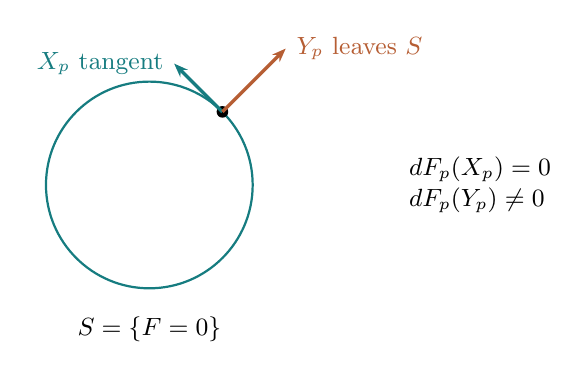
\begin{tikzpicture}[scale=1.05]
\draw[accent,thick] (0,0) circle (1.25);
\coordinate (p) at (.884,.884);
\fill (p) circle (2pt);
\draw[accent,very thick,->] (p)--(.3,1.468) node[left]{$X_p$ tangent};
\draw[warm,very thick,->] (p)--(1.65,1.65) node[right]{$Y_p$ leaves $S$};
\node at (0,-1.75){$S=\{F=0\}$};
\node[align=left] at (4,.0){$dF_p(X_p)=0$\\$dF_p(Y_p)\ne0$};
\end{tikzpicture}
\caption{The infinitesimal test is a tangency condition. It becomes a PDE symmetry test after extending the field to derivative coordinates.}
\end{figure}

For a scalar regular equation, near its zero set a symmetry may satisfy $F(g\cdot p)=a_g(p)F(p)$ with a smooth nonzero factor. Infinitesimally this permits $X(F)=\lambda F$ rather than demanding $X(F)=0$ everywhere. For differential equations the analogous relation is checked on jet space.

\section{Jet space and prolongation: making derivatives transform}\label{sec:jets}
\source{Sections 3.1--3.2, printed pp.~14--18}
\subsection{Coordinates for a function and its derivatives}
Let $\Omega\subset\R^2$ have coordinates $(x,t)$, and let $M=\Omega\times\R$ have coordinates $(x,t,u)$. The first and second jet spaces of scalar functions have coordinates
\[
J^1=(x,t,u,u_x,u_t),\qquad
J^2=(x,t,u,u_x,u_t,u_{xx},u_{xt},u_{tt}).
\]
The jet labels $u_x,u_t,\ldots$ are independent coordinates of a point of this larger space. At a fixed base point, a finite jet is a record of possible Taylor coefficients. Mixed derivatives $u_{xt}=u_{tx}$ are listed once. With $p$ independent variables, one dependent variable and order $k$,
\[
\dim J^k=p+\binom{p+k}{k}.
\]
For $p=k=2$, this is $2+6=8$. The space of order exactly $j$ derivatives has $\binom{p+j-1}{j}$ coordinates; it does not include lower orders again.

A function $U(x,t)$ gives its jet graph
\[
j^2U:(x,t)\longmapsto(x,t,U,U_x,U_t,U_{xx},U_{xt},U_{tt}).
\]
For $U=x^2+2t$, this is $(x,t,x^2+2t,2x,2,2,0,0)$. It is a two-dimensional surface. The heat equation defines a different object:
\[
\mathcal E=\{u_t-u_{xx}=0\}\subset J^2,
\]
a seven-dimensional submanifold, since $\partial(u_t-u_{xx})/\partial u_t=1$. A solution satisfies $j^2U(\Omega)\subset\mathcal E$. The equation manifold is not one solution graph and is not the infinite-dimensional space of all functions solving the PDE.

\begin{figure}[htbp]\centering
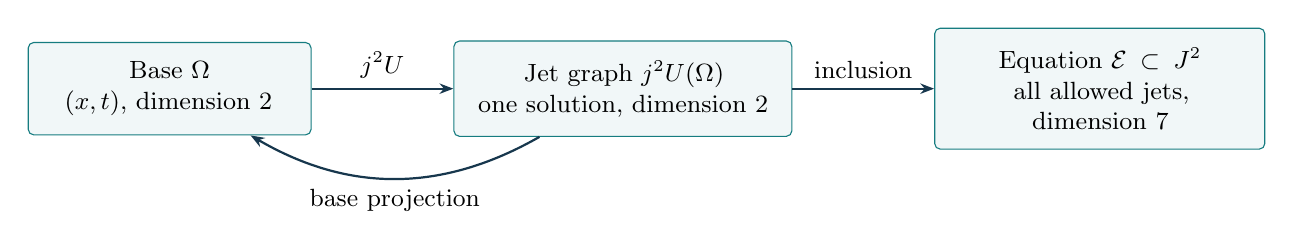
\begin{tikzpicture}[node distance=15mm and 18mm]
\node[main,text width=31mm] (b) {Base $\Omega$\\$(x,t)$, dimension 2};
\node[main,text width=38mm,right=of b] (j) {Jet graph $j^2U(\Omega)$\\one solution, dimension 2};
\node[main,text width=37mm,right=of j] (e) {Equation $\mathcal E\subset J^2$\\all allowed jets, dimension 7};
\draw[arr] (b)--node[above]{$j^2U$}(j);
\draw[arr] (j)--node[above]{inclusion}(e);
\draw[arr] (j) to[bend left=30] node[below]{base projection} (b);
\end{tikzpicture}
\caption{For the heat equation, a solution is a graph inside the equation manifold. A general surface in that manifold is not necessarily a jet graph.}
\end{figure}

\subsection{Partial derivatives versus total derivatives}\label{sec:total}
The total derivative differentiates a differential function after substitution of a graph. Formally,
\[
D_x=\partial_x+u_x\partial_u+u_{xx}\partial_{u_x}+u_{xt}\partial_{u_t}+\cdots,
\quad
D_t=\partial_t+u_t\partial_u+u_{xt}\partial_{u_x}+u_{tt}\partial_{u_t}+\cdots.
\]
If $H=H(x,t,u)$, then $D_xH=H_x+u_xH_u$. For $H=xu+u_x^2$,
\[
\partial_xH=u,\qquad D_xH=u+xu_x+2u_xu_{xx}.
\]
Substituting $u=U$, the latter equals $\partial_x[xU+(U_x)^2]$ by the usual chain rule. Generally $D_x:C^\infty(J^k)\to C^\infty(J^{k+1})$: another derivative requires another jet order. One should not treat this full operator as an ordinary vector field on a fixed finite jet space without specifying a truncation.

Jet graphs obey contact relations, for example
\[
du-u_x\,dx-u_t\,dt=0,
\quad du_x-u_{xx}\,dx-u_{xt}\,dt=0
\]
after pullback to $j^2U$. These relations enforce that the derivative labels actually come from a function. A transverse two-dimensional integral surface of the contact system is a graph locally; transversality to the base is essential.

\subsection{Derive the first prolongation from the chain rule}\label{sec:prolong}
For an ODE, let $\widetilde x=x+\varepsilon\xi(x,u)+O(\varepsilon^2)$ and $\widetilde u=u+\varepsilon\eta(x,u)+O(\varepsilon^2)$. Along a graph,
\[
\widetilde u_{\widetilde x}
=\frac{D_x\widetilde u}{D_x\widetilde x}
=\frac{u_x+\varepsilon D_x\eta+O(\varepsilon^2)}{1+\varepsilon D_x\xi+O(\varepsilon^2)}
=u_x+\varepsilon(D_x\eta-u_xD_x\xi)+O(\varepsilon^2).
\]
This proves the first prolonged coefficient. With independent variables $(x,t)$ and
$X=\xi\partial_x+\tau\partial_t+\eta\partial_u$, the general formulas are
\begin{align}
\eta^{x}&=D_x\eta-u_xD_x\xi-u_tD_x\tau,\label{eq:eta-x}\\
\eta^{t}&=D_t\eta-u_xD_t\xi-u_tD_t\tau,\label{eq:eta-t}\\
\eta^{xx}&=D_x\eta^{x}-u_{xx}D_x\xi-u_{xt}D_x\tau.\label{eq:eta-xx}
\end{align}
Use the same recursion for other derivatives:
\[
\eta^{J,i}=D_i\eta^J-\sum_a u_{J,a}D_i\xi^a.
\]
Then
\[
\pr^{(2)}X=X+\eta^x\partial_{u_x}+\eta^t\partial_{u_t}
+\eta^{xx}\partial_{u_{xx}}+\eta^{xt}\partial_{u_{xt}}+\eta^{tt}\partial_{u_{tt}}.
\]
The superscripts label coefficients, not powers or ordinary partial derivatives.

For a finite point transformation, the matrix $A_i{}^j=D_i\widetilde x^j$ must be invertible along the graph to express the transformed object as a graph over the new independent variables. A diffeomorphism of $(x,t,u)$ alone does not guarantee this for every graph: exchanging $x$ and $u$ fails where $U_x=0$. This is another reason for local domains in PDE symmetry.

\subsection{The infinitesimal PDE symmetry criterion}
For a regular equation manifold $\mathcal E=\{F=0\}\subset J^k$, impose
\begin{equation}\label{eq:criterion}
\boxed{\pr^{(k)}X(F)\big|_{\mathcal E}=0.}
\end{equation}
It says the prolonged field is tangent to the equation manifold. Local flows then preserve it and send solution graphs to solution graphs wherever the graph condition holds. For the converse statement based solely on preservation of actual solutions, a local-solvability hypothesis is needed: the permitted jets should be realized by solutions. Heat and the elementary examples here meet the usual hypotheses; singular or overdetermined systems require separate checking. Infinitesimal tests determine the identity component, not disconnected symmetries such as $x\mapsto-x$.

The resulting determining equations are linear in the unknown functions $\xi,\tau,\eta$ and their derivatives, even if the original PDE is nonlinear. This makes finding continuous point symmetries systematic. A polynomial ansatz may find useful generators but does not prove that none exist outside that ansatz.

\section{Three ways to use a symmetry}\label{sec:methods}
\source{Section 3.3}
\subsection{Canonical coordinates for a first-order ODE}\label{sec:canonical}
For a nonzero field $X=\xi\partial_x+\eta\partial_y$, seek coordinates $r(x,y),s(x,y)$ satisfying
\[
X(r)=0,\qquad X(s)=1,\qquad
\det\frac{\partial(r,s)}{\partial(x,y)}\ne0.
\]
Then the chain rule gives $X=X(r)\partial_r+X(s)\partial_s=\partial_s$. Locally its flow is translation in $s$. If $y'=f(x,y)$ and $r$ varies along a solution curve,
\[
\frac{ds}{dr}=\frac{s_x+s_yf}{r_x+r_yf}.
\]
For a symmetry this expression becomes a function of $r$ alone, so it can be integrated. The nonzero denominator is a separate transversality condition. Curves with $r$ constant can be exceptional solutions and must be checked directly. One symmetry of a higher-order ODE typically lowers its order once; complete integration requires enough appropriate symmetries, not merely a solvable algebra of any dimension.

\subsection{Transform a known solution}\label{sec:transform}
Given $U(x,t)$ and a finite symmetry
\[
(\widetilde x,\widetilde t,\widetilde u)
=(\chi_\varepsilon(x,t),\vartheta_\varepsilon(x,t),\psi_\varepsilon(x,t,u)),
\]
first substitute $u=U(x,t)$ in the last component. Then invert the first two components and express the result as $V(\widetilde x,\widetilde t)$. This inversion is essential. For space translation $(\widetilde x,\widetilde t,\widetilde u)=(x+a,t,u)$,
\[
V(\widetilde x,\widetilde t)=U(\widetilde x-a,\widetilde t).
\]
The plus sign in the point map becomes a minus sign in the argument of the transformed function.

\subsection{Select invariant solutions and reduce a PDE}\label{sec:reduction}
For a graph $u=U(x,t)$, tangent directions are $\partial_x+U_x\partial_u$ and $\partial_t+U_t\partial_u$. The field $X$ is tangent to it exactly when
\begin{equation}\label{eq:isc}
\boxed{Q=\eta-\xi U_x-\tau U_t=0\quad\hbox{on the graph}.}
\end{equation}
This invariant-surface condition is an additional equation imposed on the desired solutions. Find invariants from the characteristic ODEs
\[
\frac{dx}{ds}=\xi,\quad\frac{dt}{ds}=\tau,\quad\frac{du}{ds}=\eta.
\]
The notation $dx/\xi=dt/\tau=du/\eta$ abbreviates these ODEs. It is not permission to divide by zero: if $\eta=0$, use $du/ds=0$ directly.

Where $X\ne0$ on three-dimensional $(x,t,u)$-space, the flow-box theorem gives two independent \emph{local} first integrals. To obtain a useful graph ansatz, choose one as a reduced independent variable $z$ and the other as a dependent invariant $w$, checking that $w=F(z)$ solves locally for $u$. If a projectable $r$-parameter action has independent rank-$r$ orbits on a $p$-dimensional base and the graph/transversality conditions hold, invariant solutions can depend on $p-r$ independent variables. The relevant number is orbit rank, not the number of named generators or group parameters alone.

\begin{example}[A symmetry that removes no independent variable]
For heat, $X=\partial_u$ is a symmetry because a constant can be added to any solution. But~\eqref{eq:isc} becomes $1=0$. No graph is invariant under the whole vertical-translation group. For $X=u\partial_u$, it becomes $U=0$, selecting only the zero solution. Neither produces the usual one-variable similarity family.
\end{example}

\begin{idea}{A calculation procedure to reuse}
\begin{enumerate}
\item Write the PDE as $F(x,t,u,u_x,u_t,\ldots)=0$ and state its domain.
\item Choose a candidate field or solve the determining equations for all point fields.
\item Prolong the field and check~\eqref{eq:criterion}.
\item Check any boundary, initial and parameter restrictions of the actual problem.
\item Solve the characteristic ODEs and verify independence of the invariants.
\item Write an invariant graph ansatz; calculate every required derivative by the chain rule.
\item Substitute into the PDE, solve or approximate the reduced equation, and recover $U(x,t)$.
\item Substitute the final formula into the original PDE and data. Revisit any divided-out factors to recover exceptional branches.
\end{enumerate}
\end{idea}

\section{A nonlinear ODE: carry the reduction through}\label{sec:ode}
\source{Section 4.1, printed pp.~20--22}
Consider
\begin{equation}\label{eq:source-ode}
y'=\frac{x^2y-x+y^3-y}{x^3+xy^2-x+y}.
\end{equation}
Write $r^2=x^2+y^2$ and abbreviate
\[
N=y(r^2-1)-x,\qquad D=x(r^2-1)+y,
\quad y'=N/D\quad(D\ne0).
\]
Instead of expanding a long polynomial, observe the planar direction field
\[
W=D\partial_x+N\partial_y
=(r^2-1)(x\partial_x+y\partial_y)+(y\partial_x-x\partial_y).
\]
Both its radial and rotational components are preserved by rotations. Hence rotations map its integral curves to integral curves; on patches with $D\ne0$ these are graphs solving~\eqref{eq:source-ode}. A symmetry generator is $X=-y\partial_x+x\partial_y$. The report's linear ansatz also finds this generator; that ansatz does not classify all possible smooth symmetries of a first-order ODE.

Solve $X(r)=0$ by the characteristic equations $\dot x=-y$, $\dot y=x$:
\[
\frac{d}{ds}(x^2+y^2)=2x(-y)+2y(x)=0.
\]
Choose $r=\sqrt{x^2+y^2}>0$. On a local angular chart choose $\theta=\arg(x+iy)$; for $x>0$, $\theta=\arctan(y/x)$. Then
\[
r_x=x/r,\quad r_y=y/r,\quad
\theta_x=-y/r^2,\quad\theta_y=x/r^2,
\]
so $X(r)=0$, $X(\theta)=1$, and
\[
\det\frac{\partial(r,\theta)}{\partial(x,y)}=\frac1r\ne0.
\]
These are canonical coordinates with $X=\partial_\theta$.

Along a solution graph,
\begin{align*}
\frac{dr}{dx}&=\frac{x+y(N/D)}r
=\frac{xD+yN}{rD}
=\frac{r(r^2-1)}D,\\
\frac{d\theta}{dx}&=\frac{-y+x(N/D)}{r^2}
=\frac{xN-yD}{r^2D}=-\frac1D.
\end{align*}
Here the cancellations $xD+yN=r^2(r^2-1)$ and $xN-yD=-r^2$ supply the omitted algebra. For $r\ne1$,
\[
\frac{d\theta}{dr}=\frac1{r(1-r^2)}
=\frac1r+\frac{r}{1-r^2}.
\]
Integrating by elementary substitutions yields
\begin{equation}\label{eq:ode-solution}
\boxed{\theta=\log r-\tfrac12\log|1-r^2|+C
=\tfrac12\log\left|\frac{r^2}{1-r^2}\right|+C.}
\end{equation}
On $x>0$ this gives
\[
\boxed{\arctan(y/x)=\frac12\log\left|\frac{x^2+y^2}{1-x^2-y^2}\right|+C.}
\]
The factor $1/2$ is missing in the report's final Cartesian expression. Changing $C$ rotates the solution curve. For $r\to\infty$, $\theta\to C$ on a consistent angular branch.

\begin{figure}[htbp]\centering
\begin{tikzpicture}
\begin{axis}[width=.64\linewidth,height=6cm,axis equal image,axis lines=middle,xlabel={$x$},ylabel={$y$},xmin=-3,xmax=3,ymin=-3,ymax=3,tick label style={font=\scriptsize}]
\addplot[gray,dashed,domain=0:360,samples=100] ({cos(x)},{sin(x)});
\addplot[accent,thick,domain=1.015:3,samples=200,variable=\r] ({\r*cos(deg(.5*ln(\r^2/(\r^2-1))))},{\r*sin(deg(.5*ln(\r^2/(\r^2-1))))});
\addplot[warm,thick,domain=1.015:3,samples=200,variable=\r] ({\r*cos(deg(.5*ln(\r^2/(\r^2-1))+1.2))},{\r*sin(deg(.5*ln(\r^2/(\r^2-1))+1.2))});
\end{axis}
\end{tikzpicture}
\caption{Two exterior solution-curve portions from~\eqref{eq:ode-solution}, for $C=0$ and $C=1.2$. They differ by rotation. The dashed unit circle is an exceptional integral curve. Each plotted curve is a solution graph only on patches where $D\ne0$.}
\end{figure}

\begin{idea}{Recover the branch lost by division}
We divided by $r^2-1$. The omitted branch $r=1$ is a genuine integral curve: $x^2+y^2=1$ gives $y'=-x/y$, and $N/D=-x/y$ on that circle wherever $y\ne0$. Its upper and lower arcs are additional local graph solutions. The origin is excluded because both numerator and denominator in~\eqref{eq:source-ode} vanish there. Never discard such branches without checking them.
\end{idea}

\section{The heat equation: derive every point generator}\label{sec:heat}
\source{Section 4.2, printed pp.~22--25. The coefficient equations below replace the inconsistent signs in the report}
We seek all smooth local point fields
\[
X=\xi(x,t,u)\partial_x+\tau(x,t,u)\partial_t+\eta(x,t,u)\partial_u
\]
for $\Delta=u_t-u_{xx}=0$. Work on an open coordinate region, with no boundary or initial data imposed yet.

\subsection{Step 1: compute the prolonged coefficients}
For legibility set $p=u_x$, $q=u_t$, $r=u_{xx}$ and $s=u_{xt}$ temporarily. Equations~\eqref{eq:eta-x}--\eqref{eq:eta-t} give
\begin{align*}
\eta^t&=\eta_t+(\eta_u-\tau_t)q-\xi_t p-\xi_upq-\tau_uq^2,\\
\eta^x&=\eta_x+(\eta_u-\xi_x)p-\tau_xq-\xi_up^2-\tau_upq.
\end{align*}
For example, $D_t\xi=\xi_t+q\xi_u$, with a plus sign from the chain rule; the minus appears when multiplying by $-p$ in~\eqref{eq:eta-t}. Applying $D_x$ once more and subtracting $rD_x\xi+sD_x\tau$ gives
\begin{align}
\eta^{xx}={}&\eta_{xx}+(2\eta_{xu}-\xi_{xx})p+(\eta_{uu}-2\xi_{xu})p^2-\xi_{uu}p^3\notag\\
&-\tau_{xx}q-2\tau_{xu}pq-\tau_{uu}p^2q\notag\\
&+(\eta_u-2\xi_x)r-3\xi_upr-\tau_uqr-2\tau_xs-2\tau_ups.
\label{eq:full-heat-prolong}
\end{align}
The last two signs are negative in $\eta^{xx}$. They become positive when it is subtracted in $\eta^t-\eta^{xx}$.

\subsection{Step 2: impose tangency and split independent jets}
The invariance residual is $\pr^{(2)}X(\Delta)=\eta^t-\eta^{xx}$. Substitute $q=r$ only after computing prolongation. The $q^2$ and $qr$ terms cancel. The result is
\begin{align}
0={}&\eta_t-\eta_{xx}
+(-\xi_t-2\eta_{xu}+\xi_{xx})p
+(-\eta_{uu}+2\xi_{xu})p^2+\xi_{uu}p^3\notag\\
&+(2\xi_x-\tau_t+\tau_{xx})r
+(2\xi_u+2\tau_{xu})pr+\tau_{uu}p^2r
+2\tau_xs+2\tau_ups.
\label{eq:heat-residual}
\end{align}
On the heat equation manifold, $p,r,s$ can vary independently at a point. The coefficient functions depend only on $(x,t,u)$, so every coefficient of this polynomial in $p,r,s$ must vanish. Start with $ps$ and $s$:
\[
\tau_u=0,\quad\tau_x=0\quad\Longrightarrow\quad\tau=\tau(t).
\]
Then the $pr$ coefficient gives $\xi_u=0$, so $\xi=\xi(x,t)$. The remaining independent equations reduce to
\begin{equation}\label{eq:heat-determining}
\boxed{2\xi_x=\tau_t,\quad \eta_{uu}=0,\quad
2\eta_{xu}=\xi_{xx}-\xi_t,\quad \eta_t=\eta_{xx}.}
\end{equation}
There is no assumption that the Jacobian of every coefficient function has constant rank. Rank regularity is used for the equation manifold, while splitting uses independence of jet coordinates.

\subsection{Step 3: solve the determining equations completely}
Integrate $2\xi_x=\tau'(t)$ with respect to $x$:
\[
\xi=\tfrac12\tau'(t)x+\sigma(t).
\]
Integrate $\eta_{uu}=0$ twice with respect to $u$:
\[
\eta=A(x,t)u+B(x,t).
\]
Since $\xi_{xx}=0$, the third equation in~\eqref{eq:heat-determining} becomes
\[
2A_x=-\tfrac12\tau''(t)x-\sigma'(t),
\]
and hence
\begin{equation}\label{eq:heat-A}
A=-\tfrac18\tau''(t)x^2-\tfrac12\sigma'(t)x+\rho(t).
\end{equation}
Now $\eta_t=\eta_{xx}$ implies two equations by splitting the independent coordinate $u$:
\[
B_t=B_{xx},\qquad A_t=A_{xx}.
\]
The second is
\[
-\tfrac18\tau'''x^2-\tfrac12\sigma''x+\rho'=-\tfrac14\tau''.
\]
Split the powers of $x$:
\[
\tau'''=0,\qquad\sigma''=0,\qquad\rho'=-\tfrac14\tau''.
\]
Thus $\tau=a_0+a_1t+a_2t^2$, $\sigma=b_0+b_1t$, $\rho=-a_2t/2+c_0$, and
\begin{align*}
\tau&=a_0+a_1t+a_2t^2,\\
\xi&=(a_1/2+a_2t)x+b_0+b_1t,\\
\eta&=(-a_2x^2/4-b_1x/2-a_2t/2+c_0)u+B(x,t),\qquad B_t=B_{xx}.
\end{align*}
The arbitrary constant in $\rho$ must be retained. Rescale constants by $a_0=c_1$, $a_1=2c_2$, $a_2=4c_3$, $b_0=c_4$, $b_1=2c_5$, $c_0=c_6$. The answer is
\[
\boxed{X=\sum_{i=1}^6 c_iX_i+X_B,\qquad X_B=B(x,t)\partial_u,\quad B_t=B_{xx},}
\]
where
\begin{align}
X_1&=\partial_t,& X_2&=x\partial_x+2t\partial_t,\notag\\
X_3&=4xt\partial_x+4t^2\partial_t-(x^2+2t)u\partial_u,\label{eq:heat-basis}\\
X_4&=\partial_x,&X_5&=2t\partial_x-xu\partial_u,&X_6&=u\partial_u.\notag
\end{align}
Equation~\eqref{eq:heat-basis} is a basis for the six-dimensional part. The entire point-symmetry algebra is infinite-dimensional because any heat solution $B$ can be added to another one. This infinite family is an abelian ideal. Solving the determining equations has also explained \emph{where} the six fields in Example 2.25 came from.

\subsection{Step 4: recompute Example 2.25}\label{sec:heat-brackets}
Write the fields as triples in the fixed coordinate order $(x,t,u)$:
\[
X_1=(0,1,0),\quad X_2=(x,2t,0),\quad X_3=(4xt,4t^2,-(x^2+2t)u),
\]
\[
X_4=(1,0,0),\quad X_5=(2t,0,-xu),\quad X_6=(0,0,u).
\]
Apply~\eqref{eq:bracket}: act on the second field's coefficients, subtract its action on the first field's coefficients, then recognize the resulting triple.

For $[X_2,X_3]$, the three coefficient calculations are
\begin{align*}
X_2(4xt)-X_3(x)&=(4xt+8xt)-4xt=8xt,\\
X_2(4t^2)-X_3(2t)&=16t^2-8t^2=8t^2,\\
X_2(-(x^2+2t)u)-X_3(0)&=-2x^2u-4tu.
\end{align*}
Therefore
\[
[X_2,X_3]=8xt\partial_x+8t^2\partial_t-2(x^2+2t)u\partial_u=2X_3.
\]
The calculation on printed page 11 of the report actually computes this bracket, despite labeling it $[X_4,X_6]$ and ending with $2X_6$.

All brackets involving $X_1=\partial_t$ are obtained by differentiating coefficients in $t$:
\begin{align*}
[X_1,X_2]&=2\partial_t=2X_1,\\
[X_1,X_3]&=4x\partial_x+8t\partial_t-2u\partial_u=4X_2-2X_6,\\
[X_1,X_4]&=0,\qquad [X_1,X_5]=2\partial_x=2X_4,\qquad [X_1,X_6]=0.
\end{align*}
Similarly $[\partial_x,Y]$ differentiates the coefficients of $Y$ in $x$:
\begin{align*}
[X_2,X_4]&=-\partial_x(X_2\text{'s coefficients})=-\partial_x=-X_4,\\
[X_3,X_4]&=-4t\partial_x+2xu\partial_u=-2X_5,\\
[X_4,X_5]&=-u\partial_u=-X_6,\qquad [X_4,X_6]=0.
\end{align*}
The first two signs correct the printed table. For $[X_2,X_5]$,
\[
(X_2(2t)-X_5(x),\ X_2(0)-X_5(2t),\ X_2(-xu)-X_5(0))
=(2t,0,-xu),
\]
so $[X_2,X_5]=X_5$. For $[X_3,X_5]$, the first coefficient is $8t^2-8t^2=0$, the second is zero, and
\[
X_3(-xu)=(x^3-2xt)u
=X_5(-(x^2+2t)u).
\]
Thus this bracket also vanishes. Finally any field of the form
$a(x,t)\partial_x+b(x,t)\partial_t+h(x,t)u\partial_u$ commutes with $X_6$:
its last bracket coefficient is $X(u)-u\partial_u(hu)=hu-hu=0$, and the first two are zero. This accounts for all 15 distinct pairs.

\begin{center}\small
\setlength{\tabcolsep}{5pt}\renewcommand{\arraystretch}{1.3}
\begin{tabular}{c|cccccc}
$[\text{row},\text{column}]$ & $X_1$&$X_2$&$X_3$&$X_4$&$X_5$&$X_6$\\\hline
$X_1$&0&$2X_1$&$4X_2-2X_6$&0&$2X_4$&0\\
$X_2$&$-2X_1$&0&$2X_3$&$-X_4$&$X_5$&0\\
$X_3$&$-4X_2+2X_6$&$-2X_3$&0&$-2X_5$&0&0\\
$X_4$&0&$X_4$&$2X_5$&0&$-X_6$&0\\
$X_5$&$-2X_4$&$-X_5$&0&$X_6$&0&0\\
$X_6$&0&0&0&0&0&0
\end{tabular}
\end{center}
The real constant span is closed. Its six fields are independent: if $\sum c_iX_i=0$ on an open region, the $\partial_t$ coefficient $c_1+2c_2t+4c_3t^2$ forces $c_1=c_2=c_3=0$; the $\partial_x$ coefficient then forces $c_4=c_5=0$; the last forces $c_6=0$. Independence is as fields, not as six vectors at one point.

\subsection{Step 5: integrate all six fields}\label{sec:heat-finite}
The flow equations in Section~\ref{sec:flows} give translations, dilation and amplitude scaling immediately. The two less immediate flows deserve full integrations.

For $X_5=2t\partial_x-xu\partial_u$,
\[
\dot{\widetilde t}=0,\quad\widetilde t=t,\qquad
\dot{\widetilde x}=2t,\quad\widetilde x=x+2\varepsilon t.
\]
Then $\dot{\widetilde u}=-(x+2\varepsilon t)\widetilde u$ is a linear ODE, so
\[
\widetilde u=u\exp\left(-\int_0^\varepsilon(x+2st)\dd s\right)
=u e^{-\varepsilon x-\varepsilon^2t}.
\]
This formula also includes $u=0$. The report's $-\varepsilon t^2$ should be $-\varepsilon^2t$.

For $X_3$, define $D=1-4\varepsilon t$. First solve
\[
\dot{\widetilde t}=4\widetilde t^2\quad\Longrightarrow\quad
\widetilde t=t/D.
\]
Next $\dot{\widetilde x}=4\widetilde t\widetilde x$ integrates to $\widetilde x=x/D$. Finally
\[
\dot{\widetilde u}=-\left(\frac{x^2}{(1-4\varepsilon t)^2}+\frac{2t}{1-4\varepsilon t}\right)\widetilde u.
\]
The identities
\[
\frac{d}{d\varepsilon}\frac{\varepsilon}{1-4\varepsilon t}=\frac1{(1-4\varepsilon t)^2},
\quad
\frac{d}{d\varepsilon}\frac12\log(1-4\varepsilon t)=\frac{-2t}{1-4\varepsilon t}
\]
yield $\widetilde u=u\sqrt D\exp(-\varepsilon x^2/D)$. The real flow through zero uses $D>0$.

\begin{center}\renewcommand{\arraystretch}{1.55}
\begin{tabularx}{\linewidth}{@{}p{.11\linewidth}Y >{\raggedright\arraybackslash}p{.24\linewidth}@{}}
\toprule Field & Point transformation $(\widetilde x,\widetilde t,\widetilde u)$ & Interpretation \\
\midrule
$X_1$ & $(x,t+\varepsilon,u)$ & Time translation.\\
$X_2$ & $(e^\varepsilon x,e^{2\varepsilon}t,u)$ & Parabolic dilation.\\
$X_3$ & $\displaystyle\left(\frac{x}{D},\frac{t}{D},u\sqrt D\,e^{-\varepsilon x^2/D}\right)$ & Projective time transformation, $D>0$.\\
$X_4$ & $(x+\varepsilon,t,u)$ & Space translation.\\
$X_5$ & $(x+2\varepsilon t,t,u e^{-\varepsilon x-\varepsilon^2t})$ & Galilean transformation with amplitude factor.\\
$X_6$ & $(x,t,e^\varepsilon u)$ & Positive amplitude scaling.\\
$X_B$ & $(x,t,u+\varepsilon B(x,t))$ & Addition of a heat solution.\\
\bottomrule
\end{tabularx}
\end{center}
Each family has parameter-addition law on its domain. Composing different families is generally noncommutative. These flows generate the connected local symmetry structure; they do not enumerate disconnected symmetries such as $x\mapsto-x$ or $u\mapsto-u$. On a chosen domain such as $t>0$, impose that transformed points remain in it.

\section{Heat solutions from symmetry, with PDE checks}\label{sec:heat-solutions}
\subsection{Transform the constant solution and obtain a Gaussian}
Start with $U(x,t)=c$. Under the $X_3$ point flow, invert the first two coordinates. With $C=1+4\varepsilon\widetilde t$,
\[
x=\widetilde x/C,\quad t=\widetilde t/C,\quad D=1/C.
\]
Consequently the new solution, after renaming the independent variables, is
\begin{equation}\label{eq:heat-transform}
V(x,t)=\frac1{\sqrt{1+4\varepsilon t}}
\exp\left(\frac{-\varepsilon x^2}{1+4\varepsilon t}\right)
U\left(\frac{x}{1+4\varepsilon t},\frac{t}{1+4\varepsilon t}\right).
\end{equation}
The domain is $1+4\varepsilon t>0$ together with membership of the inverse point in the domain of $U$. The square root in the point transformation has become its reciprocal in this solution formula because the old coordinates were eliminated.

For constant $c$, take $\varepsilon>0$, $a=1/(4\varepsilon)$ and $c=\sqrt{\varepsilon/\pi}$. Then
\[
V(x,t)=\frac1{\sqrt{4\pi(t+a)}}\exp\left(-\frac{x^2}{4(t+a)}\right).
\]
The function $V(x,t-a)$ is therefore
\begin{equation}\label{eq:kernel}
\boxed{K(x,t)=\frac1{\sqrt{4\pi t}}e^{-x^2/(4t)},\qquad t>0.}
\end{equation}
Using our point-action convention, $U(x,t)\mapsto U(x,t-a)$ corresponds to the point translation $\widetilde t=t+a$. Stating the function formula avoids an ambiguous sign for ``translate in time.''

Check the PDE directly:
\[
K_t=\left(-\frac1{2t}+\frac{x^2}{4t^2}\right)K,
\quad K_x=-\frac{x}{2t}K,
\quad K_{xx}=\left(-\frac1{2t}+\frac{x^2}{4t^2}\right)K.
\]
Also $\int_{\R}K(x,t)\dd x=1$ by the Gaussian integral. As $t\downarrow0$, $K(\cdot,t)$ tends to a Dirac mass in the distributional sense, not to a finite function at the origin.

For bounded continuous initial data $f$ on the full line, the convolution
\[
U(x,t)=\int_{\R}K(x-y,t)f(y)\dd y
\]
is smooth for $t>0$, satisfies $U_t=U_{xx}$, and tends to $f(x)$ at each point as $t\downarrow0$. This supplies a solution of the initial-value problem, beyond the particular similarity families. Boundary-value problems on a half-line or interval require a kernel or other construction adapted to those boundaries.

\begin{figure}[htbp]\centering
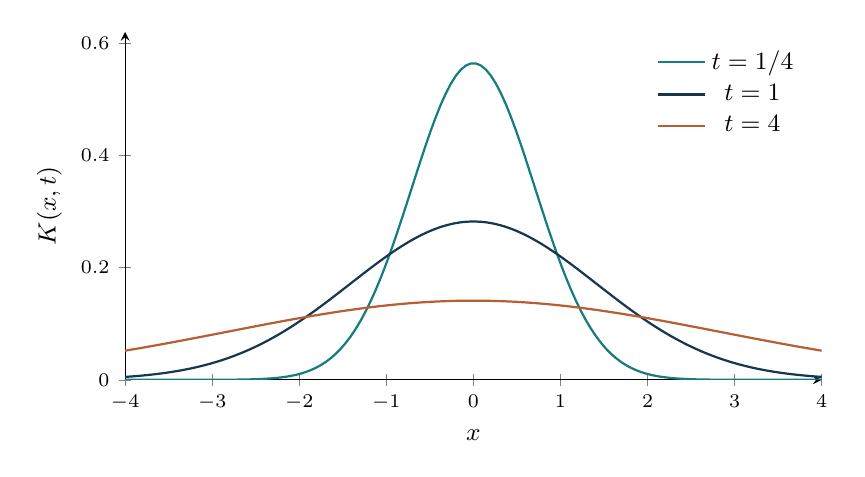
\begin{tikzpicture}
\begin{axis}[width=.86\linewidth,height=6cm,axis lines=left,xmin=-4,xmax=4,ymin=0,ymax=.62,xlabel={$x$},ylabel={$K(x,t)$},legend style={at={(.98,.98)},anchor=north east,draw=none,font=\small},tick label style={font=\scriptsize},samples=140]
\addplot[accent,thick,domain=-4:4]{exp(-x^2)/(sqrt(pi))};\addlegendentry{$t=1/4$}
\addplot[ink,thick,domain=-4:4]{exp(-x^2/4)/sqrt(4*pi)};\addlegendentry{$t=1$}
\addplot[warm,thick,domain=-4:4]{exp(-x^2/16)/sqrt(16*pi)};\addlegendentry{$t=4$}
\end{axis}
\end{tikzpicture}
\caption{The heat kernel spreads with width proportional to $\sqrt t$ while its peak decays as $t^{-1/2}$. Each full curve has unit area. The plot is generated from~\eqref{eq:kernel}, not from a schematic image.}
\end{figure}

For comparison, the $X_5$ action gives the solution formula
\[
V(x,t)=e^{-\varepsilon x+\varepsilon^2t}U(x-2\varepsilon t,t).
\]
Applied to $U=1$, it produces $e^{-\varepsilon x+\varepsilon^2t}$, not the Gaussian kernel. This separates the roles of $X_3$ and $X_5$.

\subsection{Travelling-wave reduction, including zero speed}
Choose $X=X_1+cX_4=\partial_t+c\partial_x$. The characteristic equations give
\[
\dot x=c,\quad\dot t=1,\quad\dot u=0,
\qquad z=x-ct,\quad w=u.
\]
The invariants are independent because $dz=dx-c\,dt$ and $dw=du$ are independent. An invariant graph is $U(x,t)=F(z)$. Compute
\[
U_t=-cF',\quad U_x=F',\quad U_{xx}=F''.
\]
Substituting into heat gives $F''+cF'=0$. Let $W=F'$; then $W'+cW=0$. For $c\ne0$, integrate twice and absorb constants:
\[
\boxed{U(x,t)=A+B e^{-c(x-ct)}.}
\]
For $c=0$, the correct separate family is
\[
\boxed{U(x,t)=A+Bx.}
\]
Taking $c=0$ in the first formula with fixed constants would miss the linear term. For nonzero $c$, both $U_t$ and $U_{xx}$ equal $c^2B e^{-c(x-ct)}$, verifying the PDE. If one additionally requires boundedness for all $x\in\R$, these travelling-wave families reduce to constants.

\subsection{Dilation reduction: why the variable is \texorpdfstring{$x/\sqrt t$}{x over sqrt t}}
For $X_2=x\partial_x+2t\partial_t$, restrict to $t>0$. Its flow sends $x\mapsto e^\varepsilon x$ and $t\mapsto e^{2\varepsilon}t$, so
\[
z=x/\sqrt t,\qquad w=u
\]
are invariant. Equivalently, $X_2(z)=xz_x+2tz_t=0$. Set $U=F(z)$. Since $z_x=t^{-1/2}$ and $z_t=-z/(2t)$,
\[
U_t=-\frac{z}{2t}F',\quad U_x=t^{-1/2}F',\quad U_{xx}=t^{-1}F''.
\]
Multiply the heat equation by $t$ to obtain
\[
F''+\tfrac12 zF'=0.
\]
Let $W=F'$. Then $W'/W=-z/2$ where $W\ne0$, giving $W=C e^{-z^2/4}$; the same result includes $W=0$ by $C=0$. Thus
\[
F(z)=A+B\int_0^z e^{-s^2/4}\dd s.
\]
For the half-line problem $x>0,t>0$ with $U(0,t)=1$, $U(x,0)=0$ for $x>0$, and $U\to0$ as $x\to\infty$, choose
\[
\boxed{U(x,t)=\operatorname{erfc}\!\left(\frac{x}{2\sqrt t}\right),\quad
\operatorname{erfc}(a)=\frac2{\sqrt\pi}\int_a^\infty e^{-s^2}\dd s.}
\]
This example uses the reduced ODE \emph{and} transformed boundary data to select constants. The initial and boundary values conflict at the single corner $(0,0)$, so continuity there is not asserted.

\begin{figure}[htbp]\centering
\begin{tikzpicture}
\begin{axis}[width=.79\linewidth,height=5.4cm,xmin=-3,xmax=3,ymin=0,ymax=4,axis lines=left,xlabel={$x$},ylabel={$t$},tick label style={font=\scriptsize},samples=70]
\addplot[accent,domain=.05:4,variable=\s] ({sqrt(\s)},\s);
\addplot[accent,domain=.05:4,variable=\s] ({2*sqrt(\s)},\s);
\addplot[accent,domain=.05:4,variable=\s] ({-sqrt(\s)},\s);
\addplot[accent,domain=.05:4,variable=\s] ({-2*sqrt(\s)},\s);
\addplot[ink,domain=0:4,variable=\s] (0,\s);
\node[fill=white,font=\scriptsize] at (axis cs:1.6,3.3){$z=1$};
\node[fill=white,font=\scriptsize] at (axis cs:-1.5,3.3){$z=-1$};
\end{axis}
\end{tikzpicture}
\caption{Dilation orbits in the half-plane $t>0$ have constant $z=x/\sqrt t$. An $X_2$-invariant solution has the same value along each such orbit, while different orbit labels may have different values.}
\end{figure}

\subsection{Mass-preserving similarity gives the kernel again}
Use $X_2-X_6=x\partial_x+2t\partial_t-u\partial_u$. Its independent invariants are $z=x/\sqrt t$ and $w=u\sqrt t$. Hence
\[
U(x,t)=t^{-1/2}F(z).
\]
Differentiating,
\[
U_t=t^{-3/2}(-F/2-zF'/2),\qquad U_{xx}=t^{-3/2}F''.
\]
Therefore
\[
F''+\tfrac12 zF'+\tfrac12F=0
\quad\Longleftrightarrow\quad (F'+zF/2)'=0.
\]
The integrable, decaying Gaussian branch has $F'+zF/2=0$, so $F=C e^{-z^2/4}$. Unit mass gives $C=1/\sqrt{4\pi}$ and recovers~\eqref{eq:kernel}. This second construction selects an invariant solution directly; the first constructed it by transforming a known one.

\subsection{The equation and the initial-boundary problem have different symmetries}
The PDE $U_t=U_{xx}$ is invariant under space translations. A fixed interval $0<x<L$ with fixed endpoint data generally is not. Likewise $U(x,0)=f(x)$ is changed to $f(x-a)$ by a space translation, so the original initial-value problem is preserved only if its data have the corresponding invariance.

For a boundary defined by $b(x,t)=0$, first require that the base part of the generator is tangent: $\xi b_x+\tau b_t=0$ there. Then require preservation of the boundary data, prolonging if they involve derivatives. Far-field conditions and parameter ranges must also survive. The half-line dilation above passes these checks; a generic time translation does not preserve its initial surface $t=0$.

\section{Kolmogorov: a noncommutative group and a second kernel}\label{sec:kolmogorov}
\source{Section 4.3, printed pp.~26--27. The kernel derivation here is an additional worked extension}
Consider the operator
\[
L=\partial_t-\partial_x^2-x\partial_y,\qquad LU=0.
\]
The independent-variable manifold is now $\R^3_{x,y,t}$, and the full point space includes $u$ as a fourth coordinate. Ordinary $x$-translation is not a symmetry because it changes the coefficient of $U_y$.

\subsection{Find the translations by direct substitution}
Translations in $y$ and $t$ preserve the coefficients. For an $x$-shift by $a$, compensate in $y$:
\begin{equation}\label{eq:kol-action}
(\widetilde x,\widetilde y,\widetilde t,\widetilde u)
=(x+a,y+b-at,t+c,u).
\end{equation}
The transformed function is
\[
V(\widetilde x,\widetilde y,\widetilde t)
=U(\widetilde x-a,\widetilde y-b+a(\widetilde t-c),\widetilde t-c).
\]
The chain rule gives
\[
V_{\widetilde t}=U_t+aU_y,\quad V_{\widetilde x\widetilde x}=U_{xx},\quad V_{\widetilde y}=U_y.
\]
Since $\widetilde x=x+a$, $LV=U_t-U_{xx}-xU_y=0$. Differentiating the parameters in~\eqref{eq:kol-action} gives
\[
P=\partial_x-t\partial_y,\qquad Q=\partial_y,\qquad T=\partial_t,
\quad [T,P]=-Q,\quad[P,Q]=[T,Q]=0.
\]
This is a three-dimensional nilpotent Lie algebra.

\subsection{Verify the group law and correct the exponential}
On triples define
\begin{equation}\label{eq:kol-law}
(x,y,t)\circ(a,b,c)=(x+a,y+b-at,t+c).
\end{equation}
The identity is $(0,0,0)$ and
\[
(x,y,t)^{-1}=(-x,-y-xt,-t).
\]
To check associativity, let the third triple be $(A,B,C)$. The middle coordinate of either parenthesization is
\[
y+b+B-(a+A)t-Ac,
\]
and the first and third coordinates add in the same way. The product and inverse are polynomial and therefore smooth: this is a Lie group on the manifold $\R^3$. The underlying manifold is Euclidean, but its multiplication is not vector addition.

Right translation $p\mapsto p\circ q$ is the point transformation~\eqref{eq:kol-action}. For fixed parameters these transformations compose in reverse parameter order: $R_q\circ R_r=R_{r\circ q}$. Thus they form a right action (or a left action of the opposite group); this specifies the convention instead of silently swapping sides.

A linear combination $aP+bQ+cT$ satisfies
\[
\dot{\widetilde x}=a,\quad \dot{\widetilde t}=c,\quad
\dot{\widetilde y}=b-a\widetilde t.
\]
Integrate in that order:
\begin{equation}\label{eq:kol-flow}
\boxed{\exp(\varepsilon(aP+bQ+cT))(x,y,t)
=(x+\varepsilon a,\ y+\varepsilon(b-at)-\tfrac12ac\varepsilon^2,\ t+\varepsilon c).}
\end{equation}
The $-ac\varepsilon^2/2$ term is missing if one identifies the report's combined field directly with its parameterized group law. At time one, the flow equals right translation by $(a,b-ac/2,c)$, not generally by $(a,b,c)$. Group coordinates and exponential coordinates differ.

\subsection{Anisotropic dilation and the role of the bracket}
Assign weights $w(x)=1$, $w(t)=2$. Then $\partial_t$ and $\partial_x^2$ have weight $-2$. Requiring $x\partial_y$ to have that weight gives $1-w(y)=-2$, hence $w(y)=3$. Thus
\[
\delta_\lambda(x,y,t)=(\lambda x,\lambda^3y,\lambda^2t),\qquad\lambda>0.
\]
It is a group automorphism of~\eqref{eq:kol-law}, because the product term $at$ has weight $1+2=3$. For the pullback $V=U\circ\delta_\lambda$,
\[
LV=\lambda^2(LU)\circ\delta_\lambda.
\]
Consequently it preserves the equation $LU=0$, although it rescales the operator.

The diffusion directly differentiates only in $x$. Set $Z_1=\partial_x$ and $Z_0=\partial_t-x\partial_y$. Then
\[
[Z_1,Z_0]=-\partial_y.
\]
The fields $Z_1,Z_0,[Z_1,Z_0]$ span all three tangent directions. This is the bracket-generating mechanism in H\"ormander's sufficient hypoellipticity theorem for this sum-of-squares/drift setting: the interaction with drift transfers smoothing to the missing direction. The report overstates the general theorem as a necessary-and-sufficient condition.

\subsection{Use the dilation to derive a fundamental solution}
The spatial volume $dx\,dy$ scales as $\lambda^4$, suggesting a mass-preserving amplitude of weight $-4$. Set, for $t>0$,
\[
U(x,y,t)=t^{-2}F(\xi,\zeta),\qquad \xi=x/\sqrt t,\quad\zeta=y/t^{3/2}.
\]
Direct differentiation gives
\[
U_t=t^{-3}(-2F-\tfrac12\xi F_\xi-\tfrac32\zeta F_\zeta),\quad
U_{xx}=t^{-3}F_{\xi\xi},\quad xU_y=t^{-3}\xi F_\zeta.
\]
Thus the reduced equation is
\[
F_{\xi\xi}+2F+\tfrac12\xi F_\xi+(\tfrac32\zeta+\xi)F_\zeta=0.
\]
This reduction leaves two independent variables; one symmetry did not magically turn a three-variable PDE into an ODE. Seek a Gaussian profile
\[
F=C\exp(-a\xi^2-b\xi\zeta-d\zeta^2).
\]
Divide by the positive exponential. The coefficients of $1,\xi^2,\xi\zeta,\zeta^2$ must vanish:
\[
2-2a=0,\quad4a^2-a-b=0,\quad4ab-2b-2d=0,\quad b^2-3d=0.
\]
They give $a=1$, $b=3$, $d=3$. The quadratic-form determinant is $3-9/4=3/4$, so the Gaussian integral is $2\pi/\sqrt3$. Unit spatial mass selects $C=\sqrt3/(2\pi)$ and yields
\begin{equation}\label{eq:kol-kernel}
\boxed{K_L(x,y,t)=\frac{\sqrt3}{2\pi t^2}
\exp\left(-\frac{x^2}{4t}-\frac{3(y+xt/2)^2}{t^3}\right),\quad t>0.}
\end{equation}
The coefficient equations above verify $LK_L=0$ exactly. The change of variables $(x,y)=(\sqrt t\,\xi,t^{3/2}\zeta)$ verifies unit mass and concentration at the origin as $t\downarrow0$. The tilted Gaussian shows the coupling of space and drift. For a source at $(a,b)$ at time zero, the right-translation symmetry gives the kernel $K_L(x-a,y-b+at,t)$, with its centre transported to $y=b-at$.

\section{Nonlinear PDE benchmarks from the original introduction}\label{sec:benchmarks}
The same method applies beyond heat. The examples in this section retain the original project's main models, with their parameter ranges and verification calculations made explicit. They are mathematical examples, not claims about the execution of unavailable project scripts.

\subsection{Burgers: a travelling shock calculated by quadrature}
Take $\nu>0$ and
\[
U_t+UU_x=\nu U_{xx}.
\]
The equation is invariant under translations in $x$ and $t$, so use $z=x-ct$, $U=F(z)$. Substitution gives
\[
-cF'+FF'=\nu F''\quad\Longrightarrow\quad
\nu F'=\tfrac12(F-c)^2+C.
\]
Choose $C=-k^2/2$, $k>0$, to connect the two constant states $c+k$ and $c-k$. Writing $V=F-c$, solve
\[
\frac{dV}{V^2-k^2}=\frac{dz}{2\nu},\qquad
V=-k\tanh\left(\frac{k(z-z_0)}{2\nu}\right).
\]
Hence
\begin{equation}\label{eq:burgers-shock}
\boxed{U(x,t)=c-k\tanh\left(\frac{k(x-ct-z_0)}{2\nu}\right).}
\end{equation}
To check, let $a=k/(2\nu)$ and $s=a(z-z_0)$. Then
\[
F'=-ka\operatorname{sech}^2s,\quad
F''=2ka^2\operatorname{sech}^2s\tanh s.
\]
Both $\nu F''$ and $(F-c)F'$ equal $k^2a\operatorname{sech}^2s\tanh s$. The states at $z=\mp\infty$ are $c\pm k$, and their average is the wave speed $c$. This verifies the PDE and the chosen far-field data.

\begin{figure}[htbp]\centering
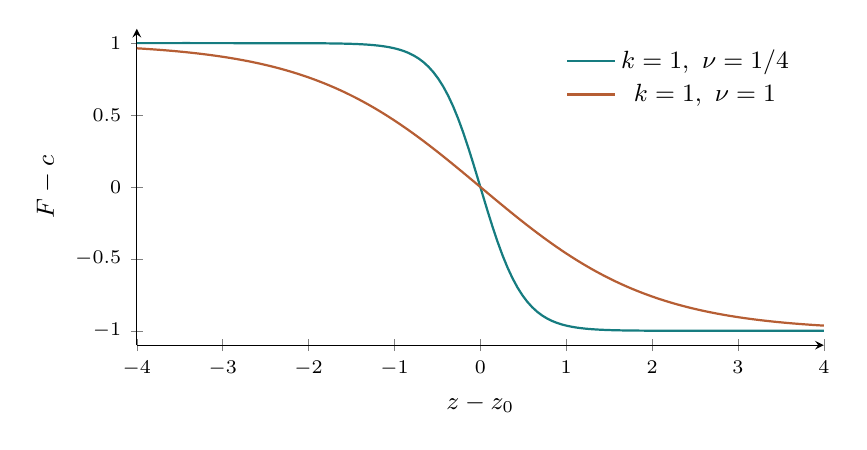
\begin{tikzpicture}
\begin{axis}[width=.85\linewidth,height=5.6cm,axis lines=left,xmin=-4,xmax=4,ymin=-1.1,ymax=1.1,xlabel={$z-z_0$},ylabel={$F-c$},samples=140,tick label style={font=\scriptsize},legend style={draw=none,font=\small,at={(.97,.97)},anchor=north east}]
\addplot[accent,thick,domain=-4:4]{-tanh(x/(2*.25))};\addlegendentry{$k=1,\ \nu=1/4$}
\addplot[warm,thick,domain=-4:4]{-tanh(x/(2*1))};\addlegendentry{$k=1,\ \nu=1$}
\end{axis}
\end{tikzpicture}
\caption{The reduced Burgers profiles. Increasing viscosity broadens the layer; the symmetry reduction determines the travelling coordinate, while integration and the end states determine the profile.}
\end{figure}

For context, its continuous point algebra for fixed nonzero $\nu$ is spanned by
\[
\partial_t,\quad\partial_x,\quad t\partial_x+\partial_u,\quad
2t\partial_t+x\partial_x-u\partial_u,\quad
 t^2\partial_t+tx\partial_x+(x-tu)\partial_u.
\]
The Cole--Hopf substitution $U=-2\nu(\log v)_x$, on a region with $v\ne0$ and a consistent logarithmic derivative, takes $v_t=\nu v_{xx}$ to Burgers. It is a differential substitution, not an ordinary point transformation of $(x,t,u)$; one should not identify the two point-symmetry algebras directly.

\subsection{Porous-medium form: a compactly supported similarity profile}
Fix $m>0$ and use the convention
\[
U_t=(U^mU_x)_x,\qquad U\ge0.
\]
This differs by an exponent shift and a constant factor from the common notation $U_t=(U^p)_{xx}$. State the convention before importing formulas. Try
\[
U=t^{-\alpha}F(z),\quad z=xt^{-\beta},\quad t>0.
\]
The derivatives are
\[
U_t=t^{-\alpha-1}(-\alpha F-\beta zF'),\quad
(U^mU_x)_x=t^{-(m+1)\alpha-2\beta}(F^mF')'.
\]
Matching powers gives $m\alpha+2\beta=1$. Finite conserved mass gives
$\int U\dd x=t^{\beta-\alpha}\int F\dd z$, so $\alpha=\beta=1/(m+2)$. The profile equation is
\[
(F^mF')'+\beta(zF)'=0.
\]
For a symmetric zero-flux profile the integration constant is zero:
\[
F^mF'+\beta zF=0.
\]
Where $F>0$, divide by $F$ and integrate:
\[
\frac1m(F^m)'=-\beta z,\qquad
\boxed{F(z)=\left(C-\frac{m\beta}{2}z^2\right)_+^{1/m},\quad C>0.}
\]
Here $(a)_+=\max(a,0)$. In the positive region the calculation verifies the PDE classically. At the moving support boundary the appropriate statement is a weak solution: the profile goes continuously to zero and the flux $F^mF'=-\beta zF$ also goes to zero. It is not generally a globally smooth classical solution across that boundary. The support expands like $t^\beta$, and the chosen mass fixes $C$.

\subsection{Fisher--KPP: reduction can succeed without elementary integration}
For
\[
U_t=U_{xx}+U(1-U),
\]
the travelling ansatz $U=F(z)$, $z=x-ct$, gives
\[
\boxed{F''+cF'+F(1-F)=0.}
\]
One seeks a decreasing front with $F(-\infty)=1$ and $F(+\infty)=0$. Set $W=F'$ to obtain the phase-plane system $F'=W$, $W'=-cW-F(1-F)$. Translational invariance of this ODE gives an order reduction, but not an automatic elementary integral. For example, where $F'\ne0$ and $W=W(F)$,
\[
W\frac{dW}{dF}+cW+F(1-F)=0
\]
is still nonlinear.

An explicit special-speed front is
\[
c=5/\sqrt6,\qquad F(z)=(1+e^{z/\sqrt6})^{-2}.
\]
To verify it, put $q=e^{z/\sqrt6}$ and $a=1/\sqrt6$. Then
\[
F'=-\frac{2aq}{(1+q)^3},\quad
F''=-\frac{2a^2q(1-2q)}{(1+q)^4},\quad
F(1-F)=\frac{q(q+2)}{(1+q)^4}.
\]
Multiplying the ODE residual by $(1+q)^4/q$ gives
\[
-2a^2(1-2q)-2ca(1+q)+(q+2)=0
\]
for $a^2=1/6$, $ca=5/6$. The end states follow by taking $q\to0$ and $q\to\infty$. Other speeds and boundary conditions lead to numerical or asymptotic profile problems; the symmetry method still supplies the reduced equation.

\section{Classification and the retained Lie-group perspective}\label{sec:classify}
\subsection{The heat algebra's structure from its table}
Let $\mathfrak h=\Span\{X_4,X_5,X_6\}$. Its only nonzero basis bracket is $[X_4,X_5]=-X_6$, so it is a Heisenberg algebra. It is an ideal in the six-dimensional algebra. Define
\[
E=X_1,\qquad F=-\tfrac14X_3,\qquad H=-X_2+\tfrac12X_6.
\]
The corrected table gives
\[
[H,E]=2E,\qquad[H,F]=-2F,\qquad[E,F]=H.
\]
Thus these fields form $\mathfrak{sl}_2(\R)$, and the finite part decomposes as
\[
\mathfrak{sl}_2(\R)\ltimes\mathfrak h_3.
\]
This describes the Lie algebra. Global group quotients and covering groups need additional choices. The infinite superposition ideal is still present in the full heat point algebra. Calling all heat symmetries a six-dimensional group would omit it.

\subsection{An optimal system is a classification up to conjugacy}
An invariant solution is usually selected by a subalgebra, and different choices can be related by a symmetry. An optimal system of one-dimensional subalgebras gives one representative per conjugacy class under a stated group. Its list may contain continuous parameters; it need not be finite or purely combinatorial.

For a small example, take the abstract algebra $[D,P]=-P$. Every nonzero generator is $aD+bP$. The adjoint operations give
\[
e^{s\operatorname{ad}P}D=D+sP,\qquad
 e^{r\operatorname{ad}D}P=e^{-r}P.
\]
If $a\ne0$, choose $s=-b/a$ to remove $P$ and rescale the generator to $D$. If $a=0$, rescale to $P$. There are two representatives, $\Span\{D\}$ and $\Span\{P\}$. In more complicated algebras, continuous parameters can survive.

For the two-dimensional translation algebra of Fisher, the adjoint action of connected translations is trivial. The lines $\Span\{\partial_t+c\partial_x\}$ have a genuine speed parameter; the algebra's dimension does not collapse all speeds into one conjugacy class. Discrete reflection can relate signs of $c$ if it is included in the equivalence group.

After a reduction by a subalgebra $\mathfrak h$, generators in its normalizer
\[
N_\g(\mathfrak h)=\{Y:[Y,\mathfrak h]\subset\mathfrak h\}
\]
can induce symmetries on the quotient when the reduction is admissible; the algebraic candidate is $N_\g(\mathfrak h)/\mathfrak h$. A sufficiently large solvable symmetry algebra of an ODE, acting with the required independence and transversality, can allow integration by successive quadratures. Solvability by itself is not a blanket integration theorem for arbitrary PDEs or arbitrary-order ODEs.

\subsection{Matrix groups as a reference catalogue}\label{sec:catalogue}
The entry map in Section~\ref{sec:gl} makes matrix groups concrete. A standard convention calls a subgroup closed \emph{relative to} $\GL(n,\C)$ a matrix Lie group. The closed-subgroup theorem supplies its embedded manifold structure. A smooth homomorphism $\rho:G\to\GL(V)$ is a representation, namely a linear action on $V$.

\begin{center}\small\renewcommand{\arraystretch}{1.25}
\begin{tabularx}{\linewidth}{@{}p{.25\linewidth}Y p{.22\linewidth}@{}}
\toprule Group & Condition or preserved structure & Real dimension \\
\midrule
$\GL(n,\R)$ & Real invertible matrices. & $n^2$\\
$SL(n,\R)$ & Determinant one. & $n^2-1$\\
$\GL(n,\C)$ & Complex invertible matrices. & $2n^2$\\
$SL(n,\C)$ & Complex determinant one. & $2(n^2-1)$\\
$O(n),\SO(n)$ & $A^TA=I$; add $\det A=1$ for $\SO(n)$. & $n(n-1)/2$\\
$O(p,q)$ & Preserve a real form of signature $(p,q)$. & $(p+q)(p+q-1)/2$\\
$U(n),SU(n)$ & $A^*A=I$; add determinant one for $SU(n)$. & $n^2$, $n^2-1$\\
$Sp(2n,\R)$ & Preserve a nondegenerate alternating form. & $n(2n+1)$\\
$Sp(n)$ & Compact quaternionic-unitary group; a different naming convention from $Sp(2n,\R)$. & $n(2n+1)$\\
$E(n)$ & Translations and orthogonal maps: $\R^n\rtimes O(n)$. & $n(n+1)/2$\\
$\operatorname{Aff}(n)$ & Invertible affine maps $x\mapsto Ax+b$. & $n(n+1)$\\
$H_n$ & Heisenberg group; one central coordinate. & $2n+1$\\
\bottomrule
\end{tabularx}
\end{center}
$O(n),\SO(n),U(n),SU(n)$ and $Sp(n)$ are compact. $\GL(n,\R)$ and the translation group are not. For $n\ge2$, $SL(n,\R)$ is noncompact; low-dimensional trivial cases should not be obscured by a blanket table entry. $O(p,q)$ is noncompact if $p,q>0$. $O(n)$ and $\SO(n)$ have the same Lie algebra because they share their identity component. Distinct groups can therefore share infinitesimal data.

Finite groups of Lie type, such as groups over finite fields, are a separate subject from the continuous local symmetries used to derive PDE reductions. A finite group can be regarded as a zero-dimensional discrete Lie group, but it supplies no nonzero infinitesimal generators. Discrete reflection symmetries can still be useful for PDEs and ML; the infinitesimal method simply does not discover them.

\section{From reduced equations to semi-analytical methods and ML}\label{sec:ml}
This section preserves the original introduction's project direction while separating established mathematics from proposed research. The supplied source does not include the project scripts, benchmark logs or a proof of a convergence certificate. The following is therefore a workflow to implement and validate, not a report that those implementation results already exist.

\subsection{Invariant solutions and equivariant models are different targets}
For a chosen subgroup, an ansatz such as $U_\theta(x,t)=t^{-1/2}F_\theta(x/\sqrt t)$ enforces its invariant-surface condition exactly. The trainable function needs one input. It represents a restricted solution family. It does not follow that the model is equivariant under all heat symmetries, or that this family contains the solution for arbitrary initial data.

An equivariant model instead concerns a map between spaces with actions. If input data transform by $\rho_{\rm in}(g)$ and outputs by $\rho_{\rm out}(g)$, require
\[
\mathcal N\bigl(\rho_{\rm in}(g)a\bigr)
=\rho_{\rm out}(g)\mathcal N(a).
\]
These actions need not be linear. For a linear homogeneous PDE, its solution space is a vector space; for nonlinear PDEs it generally is not. Preserving the zero set of a PDE residual is weaker than requiring the residual operator itself to commute with the group. The heat operator, for instance, acquires a scaling factor under dilation.

\begin{figure}[htbp]\centering
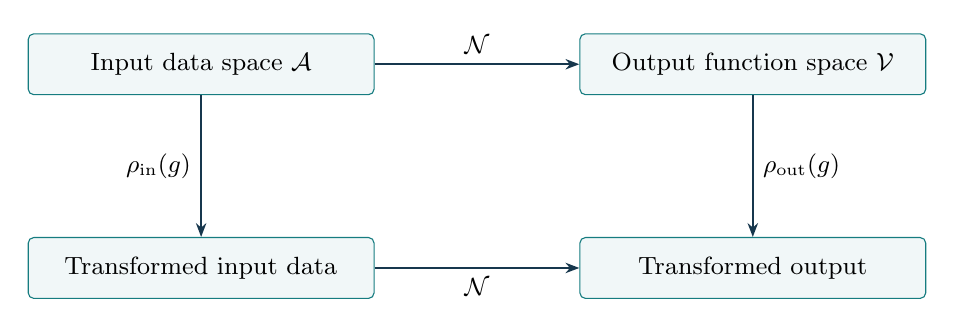
\begin{tikzpicture}[node distance=18mm and 26mm]
\node[main,text width=39mm] (a) {Input data space $\mathcal A$};
\node[main,text width=39mm,right=of a] (u) {Output function space $\mathcal V$};
\node[main,text width=39mm,below=of a] (ga) {Transformed input data};
\node[main,text width=39mm,right=of ga] (gu) {Transformed output};
\draw[arr] (a)--node[above]{$\mathcal N$}(u);
\draw[arr] (a)--node[left]{$\rho_{\rm in}(g)$}(ga);
\draw[arr] (u)--node[right]{$\rho_{\rm out}(g)$}(gu);
\draw[arr] (ga)--node[below]{$\mathcal N$}(gu);
\end{tikzpicture}
\caption{Equivariance requires the two paths to give the same output for every admissible input. This square has well-defined domains and maps; a sequence of research tasks is not by itself a commutative diagram.}
\end{figure}

\subsection{A practical research workflow}
\begin{tabularx}{\linewidth}{@{}p{.17\linewidth}Y@{}}
\toprule Stage & Concrete output and check \\
\midrule Discover & Solve determining equations, or state a restricted ansatz; verify each generator by prolongation.\\
Classify & Identify equivalent subalgebras under an explicit group; retain any continuous parameters.\\
Reduce & Derive invariants, admissibility conditions, the profile equation and transformed data.\\
Approximate & Use quadrature, an ODE solver, asymptotic series, or a stated homotopy method.\\
Estimate error & Prove an applicable stability, contraction or a-posteriori bound in a specified norm.\\
Learn a correction & Parameterize a remainder in reduced variables when the desired solution lies in that family.\\
Validate & Check original PDE residuals, boundary and initial errors, reference solutions and robustness away from training points.\\
\bottomrule
\end{tabularx}

A small residual does not automatically imply a small solution error. A useful conditional statement is: if $T$ is a contraction with constant $0<q<1$ on a complete invariant set, $U=T(U)$, and an approximation $v$ lies in that set, then
\[
\|U-v\|\le\|T(U)-T(v)\|+\|T(v)-v\|
\le q\|U-v\|+\|T(v)-v\|,
\]
so
\[
\boxed{\|U-v\|\le\frac{\|T(v)-v\|}{1-q}.}
\]
To use this as a certificate, one must construct $T$, prove its domain is preserved and bound $q$. A finite observed ratio of series terms or a symmetry algebra alone does not establish these hypotheses. Homotopy-series convergence and the effect of an ML correction require their own analysis.

\subsection{Why a symmetry penalty can add no information}
If a prolonged generator satisfies $\pr X(\Delta)=\lambda\Delta$, then a penalty based on this expression may merely duplicate the PDE residual. For translations of a differential expression with no explicit $x$, $\partial_x\Delta$ \emph{as a coordinate derivative on jet space} may be identically zero, while $D_x\Delta$ along a graph is a different operation. Confusing them can produce a vacuous loss.

A generator's usefulness depends on the loss definition, the data action and the ansatz. There is no general theorem that a zero training signal occurs exactly when an orbit has already been quotiented out. First compute the proposed loss symbolically; then check whether it imposes an independent constraint. An invariant ansatz enforces its chosen symmetry without a separate penalty but can exclude the target solution if the data are incompatible.

The useful combinatorial or algebraic tasks are commutator tables, subalgebra classification, and systematic elimination in determining equations. These organize reduction choices. They do not guarantee finite optimal systems, closed-form solutions, numerical stability or learning performance.

\section{Optional advanced language, with the limits stated}\label{sec:advanced}
This material retains the advanced topics in the original introduction as a reference layer. None is required to reproduce the calculations above. These topics describe additional structures; they do not make every PDE integrable or supply an error estimate automatically.

\subsection{Derivations, operators, and weights}
For functions, the Lie derivative along $X$ is $\mathcal L_Xf=X(f)$. In particular, $\mathcal L_{\partial_x}=d/dx$. This identifies an ordinary derivative as a special vector-field operation; it does not make every derivative a symmetry of every equation.

Let $M_x$ denote multiplication by $x$. It is an operator, not a vector field or derivation. The product rule gives
\[
[\partial_x,M_x]f=\partial_x(xf)-x\partial_xf=f,
\quad[\partial_x,M_x]=I.
\]
The quadratic differential operators
\[
E=\tfrac12M_{x^2},\quad F=-\tfrac12\partial_x^2,\quad
H=x\partial_x+\tfrac12 I
\]
satisfy $[H,E]=2E$, $[H,F]=-2F$, $[E,F]=H$. They form an operator representation of $\mathfrak{sl}_2$. Producing this triple requires quadratic and second-order operators; merely adding $x\partial_x$ to $\partial_x,M_x$ does not give this three-element algebra.

For Burgers scaling, assign $w(x)=1$, $w(t)=2$, $w(u)=-1$. A derivative subtracts the corresponding variable's weight, so
\[
w(u_t)=w(uu_x)=w(u_{xx})=-3.
\]
This verifies homogeneity. Ratios such as $x/\sqrt t$ have weight zero on appropriate domains. Similarity reduction uses such invariants and restricts to invariant graphs; it is not in general a linear projection of all solutions onto a weight-zero vector subspace. Nonlinear solution sets need not be vector spaces.

\subsection{The exponential and its analytic qualification}
The pullback of a flow acts on functions: $(\Phi_\varepsilon^*f)(p)=f(\Phi_\varepsilon(p))$. For $X=\partial_x$ this is $f(x+\varepsilon)$. It is often denoted $e^{\varepsilon X}f$. The equality
\[
f(x+\varepsilon)=\sum_{n\ge0}\frac{\varepsilon^n}{n!}f^{(n)}(x)
\]
requires analyticity and convergence in the relevant region; it is false for arbitrary smooth $f$. For example, $f(x)=e^{-1/x^2}$ for $x>0$ and $f(x)=0$ for $x\le0$ is smooth and has every derivative zero at zero, but $f(\varepsilon)>0$ for $\varepsilon>0$. The flow interpretation remains valid.

In the universal enveloping Hopf algebra, $X$ is primitive:
\[
\Delta(X)=X\otimes1+1\otimes X.
\]
In a formal power-series completion, $e^{\varepsilon X}$ is group-like:
\[
\Delta(e^{\varepsilon X})=e^{\varepsilon X}\otimes e^{\varepsilon X}.
\]
This is an algebraic counterpart of the product rule and multiplicativity of pullback. Formal completion or analytic assumptions must be specified; exponential and logarithm are not unrestricted global inverse maps. Stone--von Neumann uniqueness concerns irreducible strongly continuous unitary Heisenberg-group representations with a fixed nonzero central character. It is not a uniqueness theorem for all derivations or for the ordinary derivative on arbitrary function spaces.

\subsection{Sheaves and schemes: two different local descriptions}
A sheaf assigns data to open sets, with restriction maps and unique gluing of compatible data on an open cover. Smooth functions form a sheaf. Local solutions of a fixed differential equation also form a sheaf of sets; for a linear homogeneous equation they form a sheaf of vector spaces. A stalk records germs at a point, identifying sections that agree on some smaller neighbourhood. This language organizes local-to-global questions.

An affine scheme $\operatorname{Spec}A$ is an algebraic-geometric object constructed from a commutative ring $A$, its prime ideals, Zariski topology and structure sheaf. Ring homomorphisms correspond contravariantly to morphisms of \emph{affine} schemes; general scheme morphisms are glued locally. Polynomial models of finite jet coordinates can be described by affine schemes and polynomial equations by closed subschemes. A general smooth jet bundle is not literally an algebraic jet scheme, and a smooth PDE need not be polynomial. Algebraic jet schemes describe maps from truncated infinitesimal parameter spaces; their relation to jets of sections requires a specified algebraic setting.

\subsection{Contact geometry and prolongation}
Prolongation respects brackets:
\[
\pr^{(k)}[X,Y]=[\pr^{(k)}X,\pr^{(k)}Y].
\]
It gives a Lie-algebra action by vector fields on jet space and, by differentiation, an action on its function algebra. The induced finite action on jet coordinates is generally nonlinear. Preserving the contact system is required to send jet graphs to jet graphs, but preserving the particular PDE submanifold is an additional condition.

On $J^1$ for one scalar field over $(x,t)$, the contact distribution is the kernel of $du-u_xdx-u_tdt$. Its dimension is four, not two; a spanning set is
\[
\partial_x+u_x\partial_u,\quad\partial_t+u_t\partial_u,
\quad\partial_{u_x},\quad\partial_{u_t}.
\]
At higher finite order the distribution likewise includes the highest-order vertical directions. On infinite jet space, formal total derivatives $D_x,D_t$ span the Cartan distribution and commute. The distinction between finite and infinite jet spaces avoids incorrect dimension statements.

A differential invariant is a function $I$ of jet coordinates satisfying $\pr X(I)=0$ for the generators of the specified connected action. This does not make it automatically a highest-weight vector or Casimir. In settings satisfying appropriate algebraicity and regularity hypotheses, Lie--Tresse results give finite generation of differential invariants using invariant differentiation. Moving-frame constructions also need a suitable local cross-section, often after prolongation makes the action locally free.

\subsection{Differential modules and what they do not imply}
Let $\mathcal D$ be a ring or sheaf of linear differential operators with suitable coefficient functions. A linear equation $L(U)=0$ is encoded by the left module $\mathcal D/\mathcal D L$. Solutions with values in a chosen function space or sheaf $\mathcal F$ are described by $\operatorname{Hom}_{\mathcal D}(\mathcal D/\mathcal D L,\mathcal F)$ in the appropriate category.

The kernel of $L$ is generally not a module under \emph{all} differential operators: constants solve $\partial_x U=0$, but multiplying a nonzero constant by $x$ does not. An operator $A$ preserves the kernel if $LA=BL$ for a suitable $B$; it need not commute with $L$. A PDE point symmetry is therefore not simply the claim $[\pr X,L]=0$.

Riemann--Hilbert theory relates regular holonomic $\mathcal D$-modules on complex manifolds to constructible sheaf-theoretic objects, with the appropriate derived or perverse formulation. Flat nonsingular connections correspond to local systems, which can be described through monodromy. It is not a universal equivalence between arbitrary PDEs and representations of a fundamental group. Borel--Weil--Bott concerns representations realized through cohomology of homogeneous bundles; it does not identify arbitrary PDE solution spaces or prove numerical convergence certificates.

A diffiety is a geometric model of a suitably prolonged, formally integrable differential equation with its Cartan distribution. Differential ideals stable under total derivatives provide an algebraic description in appropriate coordinate settings. Formal integrability, regularity and the choice of category matter. None of this replaces the analytic estimate needed to control an approximation error.

\appendix
\clearpage
\section{Corrections and qualifications to the source report}\label{app:source-errors}
Page numbers in this appendix are the report's \emph{printed} page numbers; add three to obtain the PDF page number. This ledger covers the mathematical statements and computations used in the rewritten introduction. It distinguishes typographical errors, missing hypotheses and clarifications. The original report PDF is not altered.

\small
\begin{longtable}{@{}>{\raggedright\arraybackslash}p{.21\linewidth}>{\raggedright\arraybackslash}p{.73\linewidth}@{}}
\toprule Location & Correction or qualification \\
\midrule\endhead
p.~4, opening description & A manifold is locally Euclidean, not necessarily a global deformation of Euclidean space. ``Hypersurface'' means codimension one.\\
Definition 2.1 & State the topology and open chart domains explicitly; the third condition is Hausdorff separation, not another smoothness test. See Section~\ref{sec:hausdorff}.\\
Definitions 2.4--2.5 & Constant rank is not constant Jacobian entries. An immersion has injective derivative; injectivity of the map is an additional condition in the report's chosen submanifold convention.\\
Remark 2.6 & Connectedness and constant rank are hypotheses on selected objects, not properties of every manifold and smooth map. $\GL(n,\R)$ itself is disconnected.\\
Example 2.10 & The isomorphism to $\R^{n^2}$ is for the vector space $M_n(\R)$. Invertible matrices give an open subset. Smooth inversion follows from the adjugate formula. This is a clarification of what the example identifies.\\
p.~7, rotation orbit & If $c$ is the distance from the origin, the circle equation is $x^2+y^2=c^2$. The origin has a point orbit. General smooth-action orbits are immersed, not necessarily embedded.\\
p.~8, opening claim & Tangent space needs its Lie bracket to encode the local group. Global connected groups can differ by discrete quotients of their simply connected integration.\\
Definition 2.22 & Correct the repeated/mismatched indices: $(dF_pv)^j=\sum_{i=1}^{\dim M}v^i\partial_iF^j$, with $j=1,\ldots,\dim N$.\\
Definition 2.23 & The bracket is $X(Y(f))-Y(X(f))$; close the parenthesis after $Y(f)$.\\
Example 2.25, p.~10 & Replace $[X_2,X_4]=X_4$ by $-X_4$ and $[X_3,X_4]=2X_5$ by $-2X_5$. Other upper-triangle entries agree with the recomputation.\\
p.~11, worked bracket & Its actual inputs are $X_2,X_3$, and the result is $2X_3$. Replace both field labels and replace $x^2-2t$ in the final factor by $x^2+2t$.\\
p.~12, ``an algebra is a vector field'' & An algebra is a vector \emph{space} with an appropriate bilinear product. A Lie algebra uses a bracket satisfying antisymmetry and Jacobi.\\
Theorem 2.33 & Use a regular defining equation and interpret the criterion on its zero set. Infinitesimal generators determine the connected component; disconnected symmetries need finite checks.\\
Definition 2.34 & Clarification: the successive ideal condition is a subnormal flag and is equivalent to derived-series solvability in finite dimension. Each member must be an ideal in the next member, not necessarily in all of $\g$. See Section~\ref{sec:algebra}.\\
Definition 3.1 & In $\Omega\times U\times U_1\times\cdots\times U_n$, $U_j$ must contain derivatives of \emph{exactly} order $j$ to avoid counting lower orders repeatedly.\\
p.~15, solution manifold & $F=0$ is an equation manifold only under the rank hypothesis. One solution's jet graph is a smaller submanifold inside it.\\
Equation (3.4) & Evaluate $\partial_\varepsilon\widetilde x^i$ and $\partial_\varepsilon\widetilde u$ at $\varepsilon=0$ to obtain the generator at the original point.\\
Proposition 3.6 & Count mixed derivative coordinates once, or specify a symmetric-index convention. For $(x,t)$, $u_{xt}$ and $u_{tx}$ are not separate jet coordinates.\\
Theorem 3.7 & State regularity, local solvability for the solution-based converse, and the graph/transversality condition. The criterion is local and applies to connected transformations.\\
Equations (3.8)--(3.9) & The first prolonged coefficient is $\eta_x+(\eta_y-\xi_x)y'-\xi_y(y')^2$. Thus the determining equation is $\xi f_x+\eta f_y-\eta_x-(\eta_y-\xi_x)f+\xi_y f^2=0$. The sign of the $\xi_y f^2$ contribution in (3.9) is wrong.\\
Proposition 3.9 proof & The chain rule is $\partial_x=r_x\partial_r+s_x\partial_s$ and $\partial_y=r_y\partial_r+s_y\partial_s$. The printed expansion mixes these coefficients.\\
Section 3.3 & Invariant coordinates and reduction require a nonzero field, rank and graph conditions. Higher-order integration requires enough suitable symmetries. A symmetry alone does not always reduce a PDE variable.\\
Section 4.1, p.~22 & Restore the factor $1/2$ in front of the logarithm in the Cartesian implicit solution. Also recover $r=1$ solution arcs lost by dividing by $1-r^2$.\\
p.~23, prolongation & Recompute with $D_i\xi=\xi_i+u_i\xi_u$ and $D_i\tau=\tau_i+u_i\tau_u$. In particular the $\xi_tu_x$ term in $\eta^t$ is negative and the $2\tau_xu_{xt}$ term in $\eta^{xx}$ is negative. See~\eqref{eq:full-heat-prolong}.\\
Equation (4.11) & The coefficient of $u_{xx}$ must retain $-2\xi_x$ on the $\eta^{xx}$ side. After $\tau_x=0$, the relation is $2\xi_x=\tau_t$.\\
Equation (4.17) & The $x^2$ term is $-\tau_{tt}x^2/8$. Also $-\xi_t=-\tau_{tt}x/2-\sigma_t$, so both terms have minus signs before integration.\\
p.~24, constants & Integrating $\rho'=-\tau''/4$ needs an arbitrary constant. Basis fields can be rescaled; turning on one original constant need not yield the displayed normalization without that rescaling.\\
p.~24, $G_5$ & Its amplitude factor is $\exp(-\varepsilon x-\varepsilon^2t)$, not $\exp(-\varepsilon x-\varepsilon t^2)$.\\
pp.~24--25, groups & The six fields give the finite part; superposition is infinite-dimensional. Their flows generate connected local transformations, not automatically every disconnected symmetry. The Gaussian construction uses $G_3$, despite the preceding reference to $G_5$.\\
p.~25, time shift & Distinguish the point action from its action on functions. Under $\widetilde t=t+a$, the function becomes $U(x,t-a)$. Section~\ref{sec:heat-solutions} states the kernel-producing shift explicitly.\\
p.~25, travelling waves & Replace the stray variable $y$ in the intermediate exponential by the travelling coordinate. Treat $c=0$ separately to retain the stationary affine solutions.\\
p.~26, hypoellipticity & For every open $\Omega'\subset\Omega$ and distribution $u\in\mathcal D'(\Omega')$, require $Lu\in C^\infty(\Omega')\Rightarrow u\in C^\infty(\Omega')$. H\"ormander's bracket criterion in the standard theorem is sufficient; the report's blanket necessity claim is not valid.\\
p.~27, combined flow & The flow of $aP+bQ+cT$ contains $-ac\varepsilon^2/2$ in its $y$ coordinate. The displayed group law is valid, but is not the time-one exponential with the same parameters. Specify right translation as in Section~\ref{sec:kolmogorov}.\\
\bottomrule
\end{longtable}
\normalsize

\clearpage
\section{Changes to the supplied introduction}\label{app:intro-errors}
The earlier \texttt{intro.tex} contained useful conceptual and research directions, but some statements were stronger than their hypotheses allow. The current source replaces those claims rather than preserving them as teaching shortcuts.
\begin{longtable}{@{}>{\raggedright\arraybackslash}p{.35\linewidth}>{\raggedright\arraybackslash}p{.59\linewidth}@{}}
\toprule Earlier theme or claim & Treatment in this revision \\
\midrule\endhead
Every symmetry knob removes one variable & Replaced by orbit-rank and graph conditions, with vertical-translation and amplitude-scaling counterexamples. Reduction selects invariant solutions.\\
Generators are simply $T_eG$ on any $M$ & Distinguished left-invariant fields on $G$ from induced fields on $M$, including ineffective actions and the sign convention.\\
A nonlinear PDE solution space is a representation space & A general solution set is not a vector space. Use actions on sets or function spaces, and distinguish zero-set preservation from equivariance.\\
Prolongation acts linearly on jets & Jet transformations can be nonlinear. Prolongation preserves brackets and acts by derivations on functions.\\
Optimal systems are finite combinatorial lists & Some contain continuous parameters. Specify the equivalence group and calculate its adjoint orbits.\\
Solvability implies complete quadrature & Added the required number and independence of symmetries and transversality assumptions. Derived and lower-central series are separated.\\
The heat equation has only six symmetries & Kept the six-dimensional part and explicitly included the infinite superposition ideal and possible discrete symmetries.\\
All PDE groups are members of a classical catalogue & Replaced by a reference list of examples. Infinite-dimensional algebras and global covering issues prevent such a blanket assertion.\\
Schr\"odinger group as $SL(2)\ltimes$ the full Galilei group & Used the precise heat \emph{algebra} decomposition $\mathfrak{sl}_2\ltimes\mathfrak h_3$, avoiding double-counting time translations.\\
Two-dimensional conformal symmetry means every such problem is integrable & Omitted the implication. Local conformal transformations and global conformal automorphism groups are different; conformal symmetry by itself is not a general integrability theorem.\\
Derivative is the unique canonical operator by Stone--von Neumann & Stated the actual unitary-representation scope; general derivations are not uniquely determined by that theorem.\\
$e^{a\partial_x}f$ equals its Taylor series for all smooth $f$ & Distinguished flow pullback from a convergent Taylor expansion and gave a smooth nonanalytic counterexample.\\
Similarity reduction is a linear weight-zero projection & Replaced by local quotient coordinates and restriction to invariant graphs. Nonlinear solution sets do not admit the asserted vector-space projection.\\
Differential invariants are highest-weight or Casimir vectors & Removed the identification; these terms need additional representation structures and conditions.\\
All contact geometry is $\Span(D_x,D_t)$ on finite $J^k$ & Included the finite-order vertical directions and separated finite from infinite jets. A two-variable jet graph is a surface, not a curve.\\
Every smooth jet bundle is a jet scheme & Distinguished smooth and algebraic categories and jets of sections from algebraic jet schemes.\\
The kernel of a PDE operator is a $\mathcal D$-module & Replaced by the equation module $\mathcal D/\mathcal D L$ and its solution functor; supplied a counterexample to stability under all operators.\\
PDE symmetry forces commutation with $L$ & Explained the weaker intertwining relation $LA=BL$ and zero-set preservation.\\
Riemann--Hilbert identifies arbitrary PDEs with monodromy & Restricted it to the appropriate complex regular-holonomic and constructible categories.\\
Advanced algebra proves convergence certificates & Replaced by a conditional contraction estimate with explicit analytic hypotheses.\\
Unseen scripts, benchmark logs and a completed research contribution & Preserved the pipeline as proposed work. Removed assertions of prior execution or certification unsupported by the supplied files. The worked formulas here are checked directly.\\
Malformed ``commutative'' diagrams & Replaced by diagrams with defined objects, actual maps and readable captions. An informal task pipeline is labelled as such.\\
\bottomrule
\end{longtable}

\clearpage
\section{Practice questions and worked answers}\label{app:exercises}
Try each question before reading its answer. These are short checks of the concepts used in the full PDE calculations.

\begin{exercise}[Hausdorff separation]
On $S^1\subset\R^2$, how can you separate $p=(1,0)$ from $q=(-1,0)$ by open sets in the circle? Are these sets open in the plane?
\end{exercise}
\textbf{Answer.} Use $S^1\cap\{x>1/2\}$ and $S^1\cap\{x<-1/2\}$. They are disjoint, contain the respective points, and are open in the circle's subspace topology. They are not open in the plane, because they contain no two-dimensional ball.

\begin{exercise}[Rank is not the number of nonzero entries]
Compute the rank of $F(x,y)=(x+y,2x+2y,x-y)$. Does a non-square Jacobian prevent a full-rank parametrization?
\end{exercise}
\textbf{Answer.} $J_F=\left(\begin{smallmatrix}1&1\\2&2\\1&-1\end{smallmatrix}\right)$. The first and third rows form a minor of determinant $-2$, so the rank is two everywhere. It is an immersion of $\R^2$ into $\R^3$. A full-rank immersion has full \emph{column} rank, not necessarily a square Jacobian.

\begin{exercise}[A point, a tangent vector and a field]
For $X=-y\partial_x+x\partial_y$ on $S^1$, find $X_{(0,1)}$ and describe all of $T_{(0,1)}S^1$. Is $X$ itself a vector in that tangent space?
\end{exercise}
\textbf{Answer.} $X_{(0,1)}=(-1,0)$. The tangent space consists of all $(a,0)$, $a\in\R$. The field $X$ is an assignment on the whole circle; only its evaluation at $(0,1)$ lies in this particular tangent space.

\begin{exercise}[Parameter space and image]
Is $F(s)=(\cos s,\sin s)$ from $\R$ to $\R^2$ an immersion? An embedding? How does replacing the parameter space by $\R/(2\pi\mathbb Z)$ change the answer?
\end{exercise}
\textbf{Answer.} The derivative $(-\sin s,\cos s)$ never vanishes, so it is an immersion. It is not injective on $\R$, hence not an embedding. On the circle parameter space $\R/(2\pi\mathbb Z)$, the induced map is an embedding onto the unit circle.

\begin{exercise}[Matrix coordinates]
For $A=\left(\begin{smallmatrix}1&2\\0&3\end{smallmatrix}\right)$, list its coordinates and calculate its inverse. Why does this point belong to an open manifold?
\end{exercise}
\textbf{Answer.} Its coordinates are $(1,2,0,3)$ and $\det A=3$. Its inverse is $\left(\begin{smallmatrix}1&-2/3\\0&1/3\end{smallmatrix}\right)$. The nonzero-determinant condition persists under sufficiently small perturbations, because the determinant is continuous. Thus $\GL(2,\R)$ is open in the four-dimensional matrix space.

\begin{exercise}[An admissible pair]
For $\Phi_\varepsilon(q)=q/(1-\varepsilon q)$ with its flow domain $\varepsilon q<1$, calculate $\Phi_{1/4}(2)$ and ask whether $\Phi_{3/4}(2)$ belongs to the same real flow through $q=2$.
\end{exercise}
\textbf{Answer.} $\Phi_{1/4}(2)=4$. Although substituting $3/4$ into the rational expression gives $-4$, this is beyond the blow-up at $1/2$. It does not belong to the maximal solution interval containing zero. A formula having a value is not sufficient to make an action pair admissible.

\begin{exercise}[Regular map versus regular action]
Why can the rotation action map $\SO(2)\times\R^2\to\R^2$ have constant rank two while its orbit dimension changes at the origin?
\end{exercise}
\textbf{Answer.} The full action map allows the point $(x,y)$ itself to vary, and the derivative of rotation with respect to $(x,y)$ is an invertible matrix. The orbit map fixes $(x,y)$ and varies only the angle. Its velocity is $(-y,x)$, zero at the origin and nonzero elsewhere.

\begin{exercise}[Function invariance versus equation symmetry]
Let $F(x,y)=y$ and $\Phi_\varepsilon(x,y)=(x,e^\varepsilon y)$. Is $F$ invariant? Is $F=0$ invariant? What does its generator do to $F$?
\end{exercise}
\textbf{Answer.} $F\circ\Phi_\varepsilon=e^\varepsilon F$, so $F$ is not invariant as a function but its zero set is preserved. The generator is $X=y\partial_y$ and $X(F)=y=F$, which vanishes on the zero set.

\begin{exercise}[A bracket and a prolongation]
Compute $[X_4,X_5]$ for heat. Then find $\eta^x,\eta^t,\eta^{xx}$ for $X_2=x\partial_x+2t\partial_t$ and verify it is a symmetry.
\end{exercise}
\textbf{Answer.} $[\partial_x,2t\partial_x-xu\partial_u]=-u\partial_u=-X_6$. For $X_2$, $\eta=0$, $\xi=x$, $\tau=2t$, so $\eta^x=-u_x$, $\eta^t=-2u_t$, $\eta^{xx}=-2u_{xx}$. The residual is $-2(u_t-u_{xx})$, zero on the equation manifold. It need not vanish off that manifold.

\begin{exercise}[Stationary versus travelling heat solutions]
Which reduction gives every stationary heat solution on an interval? Solve it, then impose $U(0)=0$ and $U(1)=1$.
\end{exercise}
\textbf{Answer.} Use $X_1=\partial_t$, whose invariant-surface condition is $U_t=0$. Set $U=F(x)$; heat gives $F''=0$, hence $F=A+Bx$. The data select $U=x$. This is the zero-speed branch of the travelling-wave calculation.

\begin{exercise}[A nonlinear reduction check]
For Burgers, take $c=z_0=0$, $k=1$ and $\nu=1/2$ in~\eqref{eq:burgers-shock}. Verify the stationary equation.
\end{exercise}
\textbf{Answer.} $U=-\tanh x$, $U_x=-\operatorname{sech}^2x$, and $U_{xx}=2\operatorname{sech}^2x\tanh x$. Thus $UU_x=\operatorname{sech}^2x\tanh x=(1/2)U_{xx}$ and $U_t=0$.

\begin{exercise}[The Kolmogorov group is not additive]
Under~\eqref{eq:kol-law}, let $p=(1,0,0)$ and $q=(0,0,1)$. Compare $p\circ q$ and $q\circ p$. Compute the time-one flow of $P+T$ at the origin.
\end{exercise}
\textbf{Answer.} $p\circ q=(1,0,1)$ while $q\circ p=(1,-1,1)$. The group is noncommutative. Equation~\eqref{eq:kol-flow} gives $\exp(P+T)(0,0,0)=(1,-1/2,1)$, illustrating the difference between exponential and product coordinates.

\clearpage
\section{A compact calculation sheet and glossary}\label{app:sheet}
\begin{idea}{Keep these formulas beside a PDE calculation}
\begin{align*}
X&=\xi\partial_x+\tau\partial_t+\eta\partial_u,\\
[X,Y]^j&=X(Y^j)-Y(X^j),\\
D_x&=\partial_x+u_x\partial_u+u_{xx}\partial_{u_x}+u_{xt}\partial_{u_t}+\cdots,\\
\eta^i&=D_i\eta-\sum_j u_jD_i\xi^j,\\
\eta^{J,i}&=D_i\eta^J-\sum_j u_{J,j}D_i\xi^j,\\
\text{symmetry test: }&\quad\pr^{(k)}X(F)|_{F=0}=0,\\
\text{invariant graph: }&\quad\eta-\xi U_x-\tau U_t=0,\\
\text{invariants: }&\quad X(I)=0,\\
\text{flow: }&\quad\dot{\widetilde z}=X(\widetilde z),\quad\widetilde z(0)=z.
\end{align*}
Always state the domain, rank and graph hypotheses; check divided-out cases and transform the data as well as the equation.
\end{idea}

\begin{description}[style=nextline,leftmargin=0pt,labelwidth=0pt,labelindent=0pt]
\item[Atlas] Coordinate charts covering a manifold, with compatible transitions.
\item[Hausdorff] Any two distinct points admit disjoint open neighbourhoods.
\item[Product manifold] Ordered pairs of points, with product charts; dimensions add.
\item[Tangent space] All allowable first-order velocities at one fixed point.
\item[Vector field] A smooth section of the tangent bundle; a derivation on functions.
\item[Constant-rank map] A map whose derivative image dimension is constant on the specified domain.
\item[Immersion / embedding] Injective derivative / additionally a homeomorphism onto the image with its subspace topology.
\item[Lie group] A smooth manifold with a group law and smooth multiplication and inversion.
\item[Action domain] The admissible subset of pairs $(g,p)$ on which a local action is defined.
\item[Orbit] Points reachable by the action from a given point; its dimension need not equal the group dimension.
\item[Lie algebra] A vector space with a bilinear antisymmetric bracket satisfying Jacobi. A group algebra is $T_eG$ with its induced bracket.
\item[Jet] A finite record of a function value and derivatives at a point; jet coordinates support prolongation.
\item[Equation manifold] The regular zero set of the PDE's defining functions in jet space.
\item[Solution jet graph] The lift of one actual function and its derivatives; it must lie inside the equation manifold.
\item[Prolongation] The chain-rule extension of a transformation or generator to derivative coordinates.
\item[Determining equations] The linear equations for unknown generator coefficients obtained by the infinitesimal symmetry test.
\item[Invariant function] A function constant along group orbits; infinitesimally, $X(I)=0$ for the connected generators.
\item[Invariant solution] A solution graph preserved by a chosen subgroup; it satisfies the invariant-surface condition.
\item[Symmetry reduction] Construction of a lower-variable equation for an admissible invariant family, not an automatic parametrization of all solutions.
\item[Optimal system] Subalgebra representatives up to a specified conjugacy action, possibly with continuous parameters.
\item[Equivariance] A map respects specified actions on its input and output spaces.
\end{description}

\clearpage
\addcontentsline{toc}{section}{References and provenance}
\begin{thebibliography}{9}
\bibitem{ohrnell} Carl \"Ohrnell, \emph{Lie Groups and PDE}, U.U.D.M. Project Report 2020:43, Uppsala University, 2020. Supplied as \texttt{FULLTEXT01 (1).pdf}. The main organization and the nonlinear ODE, heat and Kolmogorov starting equations come from this report; corrections are listed in Appendix~\ref{app:source-errors}.
\bibitem{intro-source} \emph{From Lie Symmetry to Machine Learning: a conceptual map for semi-analytical PDE solving}. Supplied \texttt{intro.tex}, undated. Its research themes are retained in Sections~\ref{sec:benchmarks}--\ref{sec:advanced}; revised claims are documented in Appendix~\ref{app:intro-errors}.
\bibitem{etingof} Pavel Etingof, \emph{18.745: Lie Groups and Lie Algebras, I}. Supplied lecture notes \texttt{lnlg.pdf}; also available from \href{https://math.mit.edu/~etingof/lnlg.pdf}{MIT}. See Lectures 1--3 for manifolds, the notes' ``regular map'' convention, groups and actions.
\bibitem{olvernotes} Peter J. Olver, \emph{Lectures on Lie Groups and Differential Equations}, 2012. \href{https://www-users.cse.umn.edu/~olver/sm.html}{Author's lecture-note index}. Chapters 1--4 provide geometry, actions, jets and symmetry criteria. In Chapter 2, Definition 2.19 specifies regular and semi-regular actions; Chapter 4 explains local solvability. The present calculations are written out independently.
\bibitem{olver} Peter J. Olver, \emph{Applications of Lie Groups to Differential Equations}, second edition, Springer, 1993. A detailed reference for prolongation, differential invariants and reduction.
\bibitem{hydon} Peter E. Hydon, \emph{Symmetry Methods for Differential Equations: A Beginner's Guide}, Cambridge University Press, 2000.
\bibitem{lee} John M. Lee, \emph{Introduction to Smooth Manifolds}, second edition, Springer, 2012. Reference for charts, tangent bundles, rank theorems and group actions.
\bibitem{hall} Brian C. Hall, \emph{Lie Groups, Lie Algebras, and Representations: An Elementary Introduction}, second edition, Springer, 2015. Reference for the matrix-group viewpoint.
\end{thebibliography}
\end{document}
